
%--------------------------------------------------------------
%document header info
\documentclass[12pt]{report}%{book}
\pagestyle{plain}
\usepackage{PennDiss}
\usepackage{graphicx,times}
\usepackage{amsmath,amsthm, amssymb, latexsym}
\usepackage{multirow}
\usepackage{xspace}

\usepackage[usenames,dvipsnames]{color}
\definecolor{ccolor}{rgb}{0.00,0.00,0.9}
\definecolor{lcolor}{rgb}{0.25,0.25,0.9}
\usepackage[pagebackref=true,linkcolor=ccolor,citecolor=ccolor,colorlinks=true]{hyperref}
%\usepackage[pagebackref=true,colorlinks=false]{hyperref}
\usepackage[sort,round]{natbib}

\usepackage{algorithm}
\usepackage{algorithmic}
\begin{document}
%% specific commands

%kronecker features

\newcommand{\Loss}{\mathcal{L}}
\newcommand{\LossZO}{\mathcal{L}_{01}}
\newcommand{\LossM}{\mathcal{L}_{\psi}}
\newcommand{\LossA}{\mathcal{L}_{\psi}}
\newcommand{\LossMAX}{\mathcal{L}^{max}_{\psi}}
\newcommand{\X}{\mathcal{X}}
\newcommand{\E}{\mathbb{E}}
\newcommand{\bw}{\mathbf{w}}
\newcommand{\bft}{\mathbf{f}}
\newcommand{\bx}{\mathbf{x}}
\newcommand{\by}{\mathbf{y}}
\newcommand{\ip}[2]{{#1}\cdot{#2}}
\newcommand{\Rgn}{\mathcal{R}}
\newcommand{\G}{\mathcal{G}}
\newcommand{\Y}{\mathcal{Y}}

\newcommand{\Ind}{\mathbf{1}}
\newcommand{\argmax}{\mathop{\arg\max}}
\newcommand{\argmin}{\mathop{\arg\min}}
\newcommand{\minimize}{\mathop{\mathbf{minimize}}}

\newcommand{\Vones}[1]{\ensuremath{\mathbf{1}_{#1}}}
\newcommand{\eqdef}{\stackrel{\rm def}{=}}

\newcommand{\out}[1]{}
\newcommand{\denselist}{\itemsep 0pt\topsep-8pt\partopsep-8pt}
\newcommand{\mypar}[1]{\noindent{\bf #1}}

\newcommand{\deriv}[2]{ \frac{\partial #1}{\partial #2} }
\newcommand{\diag}{ \mathbf{diag} }

%% paper-specific definitions:
\newcommand{\w}{\mathbf{w}}
\newcommand{\f}{\mathbf{f}}

\def\naive{na\"{\i}ve\xspace}
\def\Naive{Na\"{\i}ve\xspace}
\def\naively{na\"{\i}vely\xspace}
\def\Naively{Na\"{\i}vely\xspace}

\newcommand{\CPS}{CPS\xspace}
\newcommand{\LLPS}{LLPS\xspace}
\newcommand{\LLPSlong}{Local Linear Pictorial Structures\xspace}


% some common mathcals
\newcommand{\cH}{\mathcal{H}}
\newcommand{\cC}{\mathcal{C}}
\newcommand{\cD}{\mathcal{D}}
\newcommand{\cL}{\mathcal{L}}
\newcommand{\cX}{\mathcal{X}}
\newcommand{\cY}{\mathcal{Y}}
\newcommand{\cR}{\mathcal{R}}
\newcommand{\cE}{\mathcal{E}}
\newcommand{\cV}{\mathcal{V}}
\newcommand{\cS}{\mathcal{S}}

\newcommand{\reals}{\mathbb{R}}
\newcommand{\defn}{\triangleq}

\newcommand{\tree}{\Upsilon}
\newcommand{\attrib}[1]{ \nopagebreak{\raggedleft\footnotesize #1\par}}
\newcommand{\myquotation}[2]{{\em #1}\\\attrib{#2}}

\newcommand{\secref}[1]{\hyperref[sec:#1]{\textsection\ref{sec:#1}}}
\newcommand{\equref}[1]{\hyperref[eq:#1]{Equation~\ref{eq:#1}}}
\newcommand{\algref}[1]{\hyperref[alg:#1]{Algorithm~\ref{alg:#1}}}
\newcommand{\probref}[1]{\hyperref[prob:#1]{Problem~\ref{prob:#1}}}
\newcommand{\thmref}[1]{\hyperref[thm:#1]{Theorem~\ref{thm:#1}}}
\newcommand{\lemref}[1]{\hyperref[lem:#1]{Lemma~\ref{lem:#1}}}
\newcommand{\tabref}[1]{\hyperref[tab:#1]{Table~\ref{tab:#1}}}
\newcommand{\figref}[1]{\hyperref[fig:#1]{Figure~\ref{fig:#1}}}
\newcommand{\figreff}[2]{\hyperref[fig:#1]{Figure~\ref{fig:#1}#2}}


\newcommand{\score}[0]{s(x,y)}
\newcommand{\pscore}[0]{s^p(x,y)}
\newcommand{\mmi}[0]{s^\star_x(y_i)}
\newcommand{\witnessi}[0]{y^\star(y_i)}

%\renewcommand{\includegraphics}[2]{}

%% usual commands
\newcommand{\todo}[1]{\textcolor{red}{{\bf TODO:} #1 }}
%\newcommand{\todo}[1]{{\bf{TODO: #1}}}
%\newcommand{\todo}[1]{}

%\newtheorem{theorem}{Theorem}[section]
%\newtheorem{lemma}[theorem]{Lemma}
%\newtheorem{proposition}[theorem]{Proposition}
%\newtheorem{corollary}[theorem]{Corollary}

%\newenvironment{proof}[1][Proof]{\begin{trivlist}
%\item[\hskip \labelsep {\bfseries #1}]}{\end{trivlist}}
%\newenvironment{definition}[1][Definition]{\begin{trivlist}
%\item[\hskip \labelsep {\bfseries #1}]}{\end{trivlist}}
%\newenvironment{example}[1][Example]{\begin{trivlist}
%\item[\hskip \labelsep {\bfseries #1}]}{\end{trivlist}}
%\newenvironment{remark}[1][Remark]{\begin{trivlist}
%\item[\hskip \labelsep {\bfseries #1}]}{\end{trivlist}}

%\newcommand{\qed}{\nobreak \ifvmode \relax \else
%      \ifdim\lastskip<1.5em \hskip-\lastskip
%      \hskip1.5em plus0em minus0.5em \fi \nobreak
%      \vrule height0.75em width0.5em depth0.25em\fi}

%\newcommand{\qed}{\hfill \ensuremath{\Box}}

%\newcommand{\qed}{\ensuremath{\Box}}

\newcommand{\boxedequation}[2]{%
  \[\fbox{
      \addtolength{\textwidth}{-2\fboxsep}%
      %\addtolength{\linewidth}{-2\fboxsep}%
      \addtolength{\linewidth}{-2\fboxrule}%
      \begin{minipage}{#1\linewidth}%
      \begin{equation}#2\end{equation}%
      \end{minipage}%
    }\]%
}
\newcommand{\boxedeqnarray}[1]{%
  \[\fbox{%
      %\addtolength{\linewidth}{-2\fboxsep}%
      %\addtolength{\linewidth}{-2\fboxrule}%
      \begin{minipage}{0.7\linewidth}%
      \begin{eqnarray*}#1\end{eqnarray*}%
      \end{minipage}\nonumber%
    }\]%
}

%abbreviations
% Add a period to the end of an abbreviation unless there's one
% already, then \xspace.
\makeatletter
\DeclareRobustCommand\onedot{\futurelet\@let@token\@onedot}
\def\@onedot{\ifx\@let@token.\else.\null\fi\xspace}
%\def\eg{\emph{e.g.}}
\def\eg{\emph{e.g}\onedot} \def\Eg{\emph{E.g}\onedot}
\def\ie{\emph{i.e}\onedot} \def\Ie{\emph{I.e}\onedot}
\def\cf{\emph{c.f}\onedot} \def\Cf{\emph{C.f}\onedot}
\def\etc{\emph{etc}\onedot} \def\vs{\emph{vs}\onedot}
\def\wrt{w.r.t\onedot} \def\dof{d.o.f\onedot}
\def\etal{\emph{et al}\onedot}

%\def\ie{\emph{i.e.}}
%\makeatother


\renewcommand{\algorithmicrequire}{\textbf{Input:}} 
\renewcommand{\algorithmicensure}{\textbf{Ouput:}}

%% specific commands
\newcommand{\trans}[1]{{#1}^{\ensuremath{\mathsf{T}}}}           % transpose
\newcommand{\st}{\quad\textrm{s.t.}\quad}                        % s.t. for such that
\newcommand{\mvec}{\textrm{vec}}
\newcommand{\nchoosek}[2]{\left(\begin{array}{c}#1\\#2\end{array}\right)}  %use binom instead...

\newcommand{\mytitle}{Efficient Human Pose Estimation with Higher-order Image Information}
\newcommand{\MYTITLE}{EFFICIENT HUMAN POSE ESTIMATION WITH HIGHER-ORDER IMAGE INFORMATION}

\title{\mytitle}
\author{Benjamin John Sapp}

\copyrightyear{2012}

\supervisor{Ben Taskar}
\groupchair{Jianbo Shi}
\dept{Computer and Information Science}
  
 %%%%%%%%%%%%%%%%%%%%%%%%%%%%%%%%%%%%%%%%%%%%%%%%%%%%%%%%%%%%%%%%%%%%%%%%%%%%%%%
 \beforepreface
\newpage
\copyrightpage
\prefacesection{Acknowledgments}
I'd like to thank  \ldots

\newpage
\abstractp
Human pose estimation from monocular images is one of the most challenging and 
computationally demanding problems in computer vision. Standard models such as 
Pictorial Structures consider interactions between kinematically connected 
joints or limbs, leading to inference cost that is quadratic in the number of 
pixels. As a result, researchers and practitioners have restricted themselves 
to simple models which only measure the quality of limb-pair possibilities by 
their 2D geometric plausibility.

In this talk, we propose novel methods which allow for efficient inference in 
richer models with data-dependent interactions. First, we introduce structured 
prediction cascades, a structured analog of binary cascaded classifiers, which 
learn to focus computational effort where it is needed, filtering out many 
states cheaply while ensuring the correct output is unfiltered. Second, we 
propose a way to decompose models of human pose with cyclic dependencies into a 
collection of tree models, and provide novel methods to impose model agreement.

These techniques allow for sparse and efficient inference on the order of 
minutes per image or video clip. As a result, we can afford to model pairwise 
interaction potentials much more richly with data-dependent features such as 
contour continuity, segmentation alignment, color consistency, optical flow and 
more. We show empirically that these richer models are worthwhile, obtaining 
significantly more accurate pose estimation on popular datasets.



\afterpreface
\prefacesection{Preface}
Heyyyy preface.

%%%%%%%%%%%%%%%%%%%%%%%%%%%%%%%%%%%%%%%%%%%%%%%%%%%%%%%%%%%%%%%%%%%%%%%%%%%%%%%

\newpage
\pagenumbering{arabic}
\pagestyle{plain}

\part{Introduction}
\chapter{Introduction}
\begin{quote}
Because it's there.
\end{quote}
\hfill --- George Mallory, when asked why he wanted to climb Mount Everest.\\
\vspace{0.5in}

The idea of an intelligent robot performing a variety of tasks, extraordinary 
and mundane, up to and exceeding human performance, has captured the hearts and 
minds of people since at least the European Renaissance.  A key feature of much 
of this romantic vision is that robots can interact with {\em us}---working 
with, around and for humans.  An understanding of human pose is a crucial 
component to making this compelling dream become a reality.  

In the more practical and not-too-distant future, understanding human pose from 
images has enormous potential to help in many computer vision tasks: semantic 
indexing of images and video~\citep{posesearch}, action 
recognition~\citep{pose-action11}, human-object interaction~\citep{bangpeng12}, 
and scene understanding~\citep{gupta11}, to name a few.   

The problem of human pose understanding is also interesting in its own right.  
It pushes the boundaries of what can and cannot be accomplished by artificially 
intelligent systems.  Infants and even other species can understand human 
pose---why can't a computer?  

Pose estimation subsumes one of the holy grails of computer vision: general 
object recognition.  It serves as useful vehicle to demonstrate computer vision 
techniques that can be used in other subfields.  Humans can be considered a 
collection of related objects (body parts), or a single, highly deformable 
object.  The parts themselves are some of the most difficult to detect in the 
literature.  Typical objects that researchers work on recognizing---faces, 
bicycles or even potted plants \citep{voc09}---have distinguishing features, 
reliable patterns and limited intra-class variability.  A body part such as a 
lower arm, on the other hand, is far more generic.  It has a generic shape---
at best it can be described as a projection of a cylinder or frustum---and is 
subject to much higher intra-class variability due to clothing, articulated 
pose, body type, and severe foreshortening.  Features developed must be 
invariant to pose, lighting, texture and color and still discriminate parts 
from clutter, or efficient search procedures over these variations need to be 
developed. These types of techniques are valuable for computer vision in 
general.

Human pose estimation is also one of the most computationally demanding 
problems in computer vision, as the set of possible outputs is combinatorial in 
the number of parts.  It can be posed as a graph assignment or graphical model 
inference problem with an enormous set of possible labels (for each part, 
determine which pixel it is associated with).  This makes it an interesting 
testbed for advancements in graphical model and matching algorithms for and 
beyond computer vision.

Finally, the problem of pose estimation is timely.  In the computer vision 
community, statistical machine learning tools and supervised datasets give us 
principled protocols to learn effective recognition models which didn't exist a 
decade ago.  Robots, cameras, and automated systems are more and more pervasive 
in everyday life.  The demand for reliable pose estimation is already felt in 
the entertainment and defense industries. 

For all these reasons---practical applications, the dream of artificial 
intelligence, the general applicability to vision and machine learning, the 
convergence of technology to make it all possible---human pose estimation is an 
excellent problem upon which to focus.


\section{Problem Statement}

Here we formalize our problem definition input, output and computational 
requirements as follows:  

\begin{problem}[2D human upper-body pose estimation]
\label{prob:pose}
\hspace*{\fill}
\begin{itemize}
 \item[Input:] A single RGB image or RGB video sequence containing the rough 
location and scale of a person in every frame, with no additional information.
\item[Output:] Line segments describing the major anatomical parts \{left and 
right upper arms, left and right lower arms, torso, head\} in pixel 
coordinates.
\item[Requirements:] Computation time and space polynomial in the number of 
input pixels and number of output parts.
\end{itemize}
\end{problem}

\begin{figure}[tb]
\begin{center}
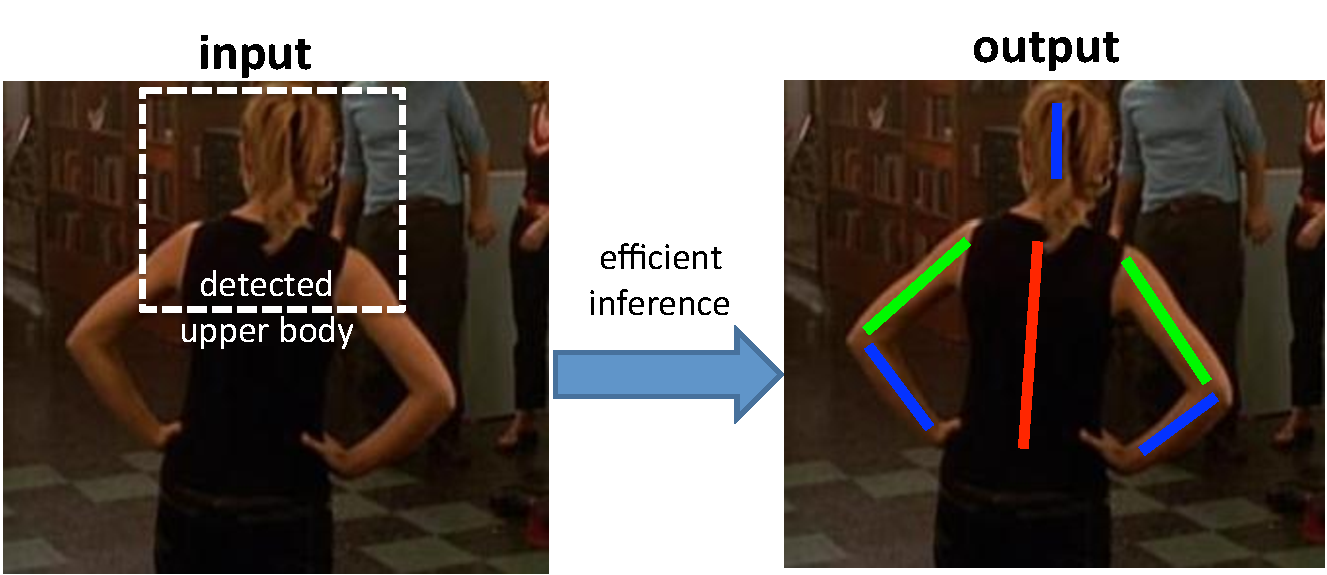
\includegraphics[width=0.95\textwidth]{figs/problem-statement.pdf}
\caption[Statement of problem.]{An example illustrating the pose estimation 
problem, formalized in~\probref{pose}.}
\label{fig:pose-problem}
\end{center}
\end{figure}

Importantly, we concern ourselves only with 2D (two dimensional) input.  This 
makes the task much more challenging than when using additional sensors, such 
as in Microsoft's Kinect capture system~\citep{kinect} where depth information 
and hence reliable knowledge of the background can be used.  However, our 
limited-sensor problem also means it can be applied in more general settings: 
we can apply such pose estimation methods outdoors and on the wealth of 
archival images and footages already stored on personal computers, libraries, 
and photo and video sharing web sites.  

Furthermore, we do not assume any additional information, such as knowledge of 
the foreground, background, clothing, lighting, indoor versus outdoor, 
etcetera.  All these factors work to confound estimation by introducing 
appearance artifacts.  We refer to our general setting as pose estimation {\em 
in the wild}, to stress the fact that the datasets we consider are from 
unconstrained foreground and backgrounds settings (or nearly unconstrained, 
when dealing with TV shows).

Also of note, we only consider the upper body, although all methods and models 
discussed in this work can be extended to full body processing (\ie including 
hips and upper and lower legs).  In fact, most of the models and tools 
developed in this work can be applied to other articulated objects, and in 
general, other domains in which estimating the instantiation of interacting 
parts (\eg, handwriting recognition, or gene sequencing). We focus on upper 
body human pose in this work because (1) most interesting pose variation occurs 
in the upper body, (2) there is a vast amount of data of people's upper bodies 
from TV shows, movies and images where lower halves are not visible, and (3) 
there is little extra knowledge to be learned about pose estimation by 
including the lower body parts, while increasing the computation time of all 
models at least linearly.  

Finally, we restrict ourselves to polynomial running time.  The space of all 
possible poses is exponential in the number of parts. The ideal approach, if 
computation were not an issue, would be to enumerate all possible poses and 
score them all using any scoring function of arbitrary complexity. However, 
this is simply not feasible, and we are forced to make conditional independence 
assumptions between certain parts to achieve tractability.  In practice, we 
wish to estimate pose on the order of a few minutes or seconds per frame.

\section{Intrinsic difficulties}
Human pose estimation in the wild is an extremely challenging problem.  It 
shares all of the difficulties of object detection, such as confounding 
background clutter, lighting, viewpoint, and scale. In addition, there are 
significant difficulties unique to human poses.  We are forced to reason over 
an enormous number of plausible poses for each image, making this a very 
computationally demanding problem.  In this section we go over the intrinsic 
difficulties of this problem, both from perceptual and computational 
standpoints.

\subsection{Perceptual issues}\label{sec:perceptual}
\begin{figure}[tb]
\begin{center}
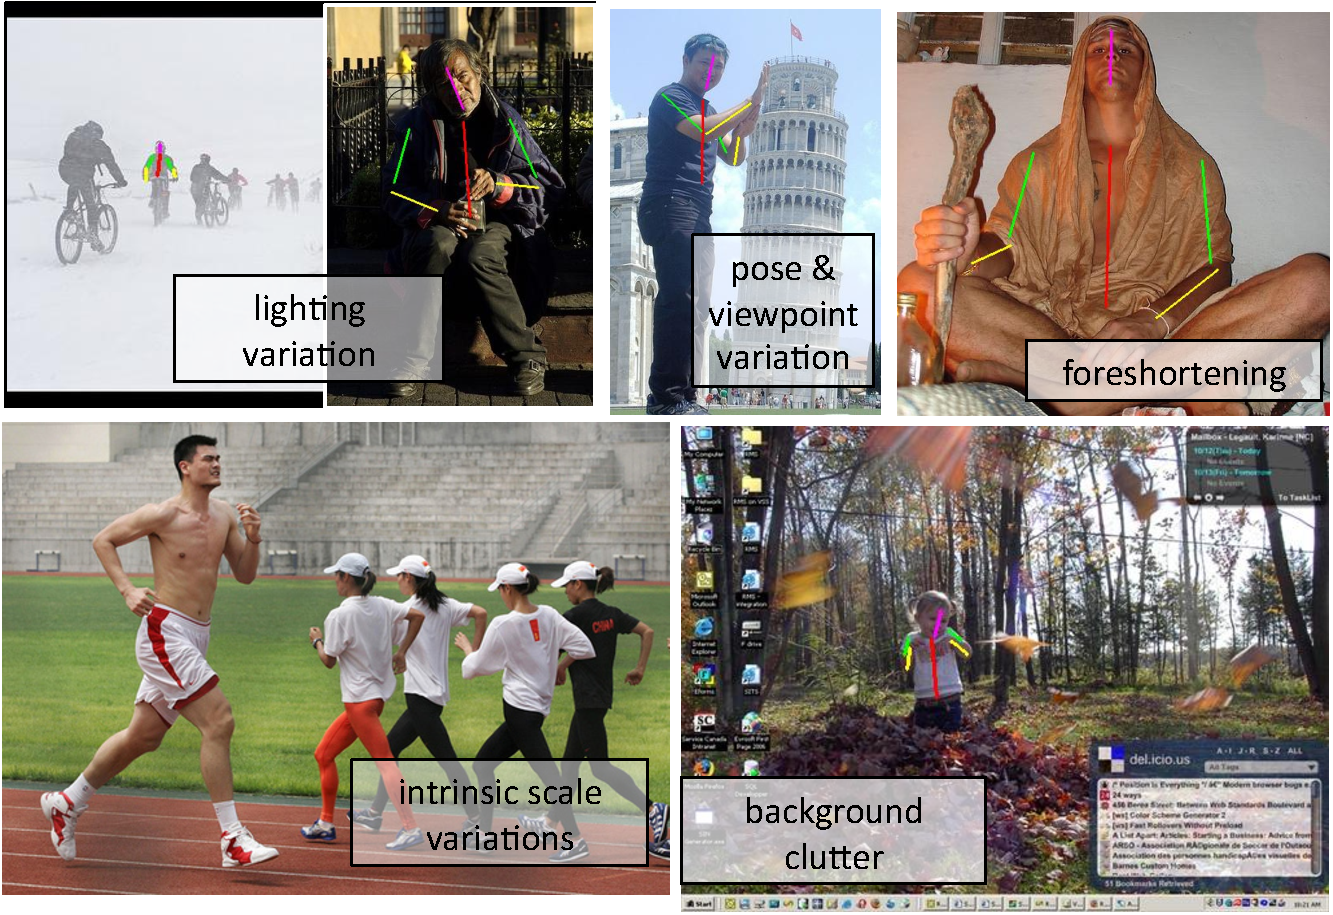
\includegraphics[width=1.05\textwidth]{figs/perceptual-issues.pdf}
\caption[Perceptual difficulties in pose estimation]{Some of the perceptual 
challenges in human pose estimation.  Large variations in lighting, pose, 
viewpoint, foreshortening, relative scale and clutter all work to confound pose 
estimation.  See~\secref{perceptual}}
\label{fig:perceptual-issues}
\end{center}
\end{figure}

One of the primary difficulties in human pose estimation is that appearance of 
pose is largely unconstrained, making it highly variable with multiple 
appearance modes.  The following issues are illustrated 
in~\figref{perceptual-issues}.

\mypar{Lighting:} Images of pose can be taken indoor or outdoor, making not 
only the mean intensity of the image variable (signal bias), but also contrast 
(signal gain). This issue is well studied in computer vision, and to an extent, 
features have been developed to be invariant to lighting, \eg, HoG~\citep{hog}, 
but require harsh quantization and local normalization of edge energy 
information. 

\mypar{Viewpoint and pose: } Humans can look very different depending on where 
they are with respect to the imaging plane.  The global ``twist'' (rotation 
about the length-of-body axis) which determines the degree of frontal versus 
profile stance of the person can be somewhat mitigated by coarse person 
detectors~\citep{andriluka2010}.  However, the body can also go through radical 
appearance changes due to the articulation of the limbs, forcing practical 
systems to decompose the modeling into the most basic, articulation-invariant 
components as atomic units: limbs and joints.

\mypar{Relative scale:} We assume our input is a detected person at a rough 
global scale.  However, we still have a large variation in the scale of parts 
in two different ways: In any particular person, the ratio of limb lengths may 
not be consistent; \eg a baby's proportions are very different than an adult's.  
Across people, there are also a large differences in the geometries of parts, 
based on gender, body type (fat, skinny, muscular), and age.  These further 
contribute to the variability in appearance.

\mypar{2D projection:} The fact that we are working with images that are 
projections of the real world lead to further difficulties.  Foreshortening 
makes estimating the length of the limb in 2D coordinates even more difficult, 
and changes the appearance.  Self-occlusions and foreground occlusions make a 
part invisible and are very hard to determine without further scene or depth 
knowledge.  Finally, it is inherently ambiguous to map from 2D pose to 3D real 
world coordinates (even up to an unknown global scale factor), discussed 
further in~\secref{limitations}.  This makes it difficult to model priors on 
arm length, as we are forced to measure and reason about lengths on the 2D 
pixel grid.

\mypar{Clothing:} Clothing contributes a near-infinite space of foreground 
variation.  Not only is clothing responsible for foreground clutter, it also 
can be considered an occluder which hides parts (\eg baggy clothing, skirts, 
ponchos) and can break assumptions about left-right appearance symmetry (\eg an 
asymmetric shirt).

\mypar{Background clutter:} Background clutter accounts for roughly half the 
errors in pose estimation performance. Often it is extremely difficult to 
separate edges in the background from lower arms.  Lower arms appear as little 
more than a pair of roughly parallel lines in an image, as do many man-made 
structures and natural objects in backgrounds: walls, tables, chairs, posts, 
trees, etcetera.

\begin{figure}[tb]
\begin{center}
\includegraphics[width=1.05\textwidth]{figs/dataset-multimodal.pdf}
\caption[Variations in appearance]{Some illustrations of variation in 
appearance in the PASCAL Stickmen dataset.  (a) An average of the dataset in 
grayscale.  (b) Average of Sobel edges over dataset.  (c) Polar histogram of 
the inner angle made between upper and lower arm, with examples for 
$0^\circ,45^\circ,90^\circ,135^\circ,180^\circ,225^\circ,270^\circ$ and 
$315^\circ$. (d) A random sampling of 100 left elbows from the Buffy Stickmen 
pose dataset,	removing color and intensity bias, to illustrate the huge variety 
of appearance due to	clutter, motion blur, clothing, body type, and pose.  
\label{fig:dataset-multimodal}}
\end{center}
\end{figure}



\subsection{Computational issues}

To operationalize \probref{pose}, let $x$ be the input image pixels, and $y$ be 
a representation of the output predicted pose.  Then a general solution 
to~\probref{pose} would take the form of a {\em scoring function} $s(x,y)$ 
which evaluates the quality of any estimated pose $y$ in the image $x$.  We can 
define the ``best'' pose as the highest scoring: $y^\star = \argmax_y s(x,y)$ 
(or $y^\star = \arg\sup_y s(x,y)$ if $y$ is infinite dimensional, \ie 
continuous).  Then~\probref{pose} is satisfied if this determination of the 
maximizer can be done in polynomial time. There are two sources of intrinsic 
computational complexity within this framework. 

\mypar{Complexity of the input:} For the reasons outlined 
in~\secref{perceptual}, there are an astronomical number of different inputs 
$x$ that can map to the same true pose $y$---the same layout of body parts can 
look very different from image to image.  The problem is inherently multimodal, 
in the sense that radically different appearances are equally valid input 
representations of any particular pose.  For a few different illustrations of 
the variability of a dataset, see~\figref{dataset-multimodal}. 

To deal with this complex problem, we are forced to either design features that 
are invariant to the multimodality (\eg, a generic patch-based arm detector 
based on coarse edges, or geometric features based on relative part coordinate 
systems), or to partition the space and model multiple modes separately.  In 
the case of the latter approach, we are faced with other difficult decisions 
regarding model complexity: how to define modes and a notion of locality, and 
what the right trade-off is between the richness of the model and the error in 
fitting the model at different modes with a finite amount of training data.

\mypar{Complexity of the output:}
The enormous combinatorial space of possible output poses is a second source of 
computational complexity.  A typical discretization of the state space of human 
poses is an $80 \times 80$ spatial grid of part locations at $24$ possible 
angles~\citep{felz05}, resulting in an output space that is roughly $150000$ 
possibilities for each part, and thus $150000^6 \approx 10^{30}$ for the joint 
output space of all $6$ upper body parts~\footnote{In the case of continuous 
spaces, the output space is infinite (infinitely precise), and to maintain 
tractability the form of $s(x,y)$ is typically analytical with a closed-form 
maximum, mean and/or mode, or approximate sampling techniques are used for 
inference. See \secref{rel}.}.

Enumerating all possibilities for a joint configuration of all parts is clearly 
not feasible.  At the other extreme, we could ignore part interactions, and 
estimate the pose of each part separately---a task which instead has $6 \times 
150000$ possibilities, which is computationally very cheap with modern 
computers.  However, individual part detection is extremely difficult for body 
parts~\citep{andriluka09} due to the wide range of appearances and lack of 
discriminating features.

Between the two extremes of (1) estimating parts in isolation and (2) 
enumerating all possible joint pose configurations, there lies a family of 
models $s(x,y)$ that consider {\em some} part interactions, but not all.  The 
simplest of these is a {\em first-order}, or {\em pairwise model}, which looks 
at pairs of part interactions at a time, and the graph of part interactions 
forms a tree structure.  This compromise between a full model of every part and 
a decoupled model of independent parts will be the basic model building block 
throughout this work.

In such a pairwise model, the basic bottleneck operation is to evaluate the 
quality of a pair of parts at a time. The model combines all such pairwise 
scores together to determine the optimal global pose.  This scoring requires 
$150000^2 \approx 1$ billion possibilities to consider for a pair of parts in 
our example $80 \times 80 \times 24$ state space, which is large but just small 
enough for modern machines to handle with some additional model restrictions, 
detailed in~\secref{ps}.


\section{Contributions of this thesis}
\begin{figure}[t!]
\begin{center}
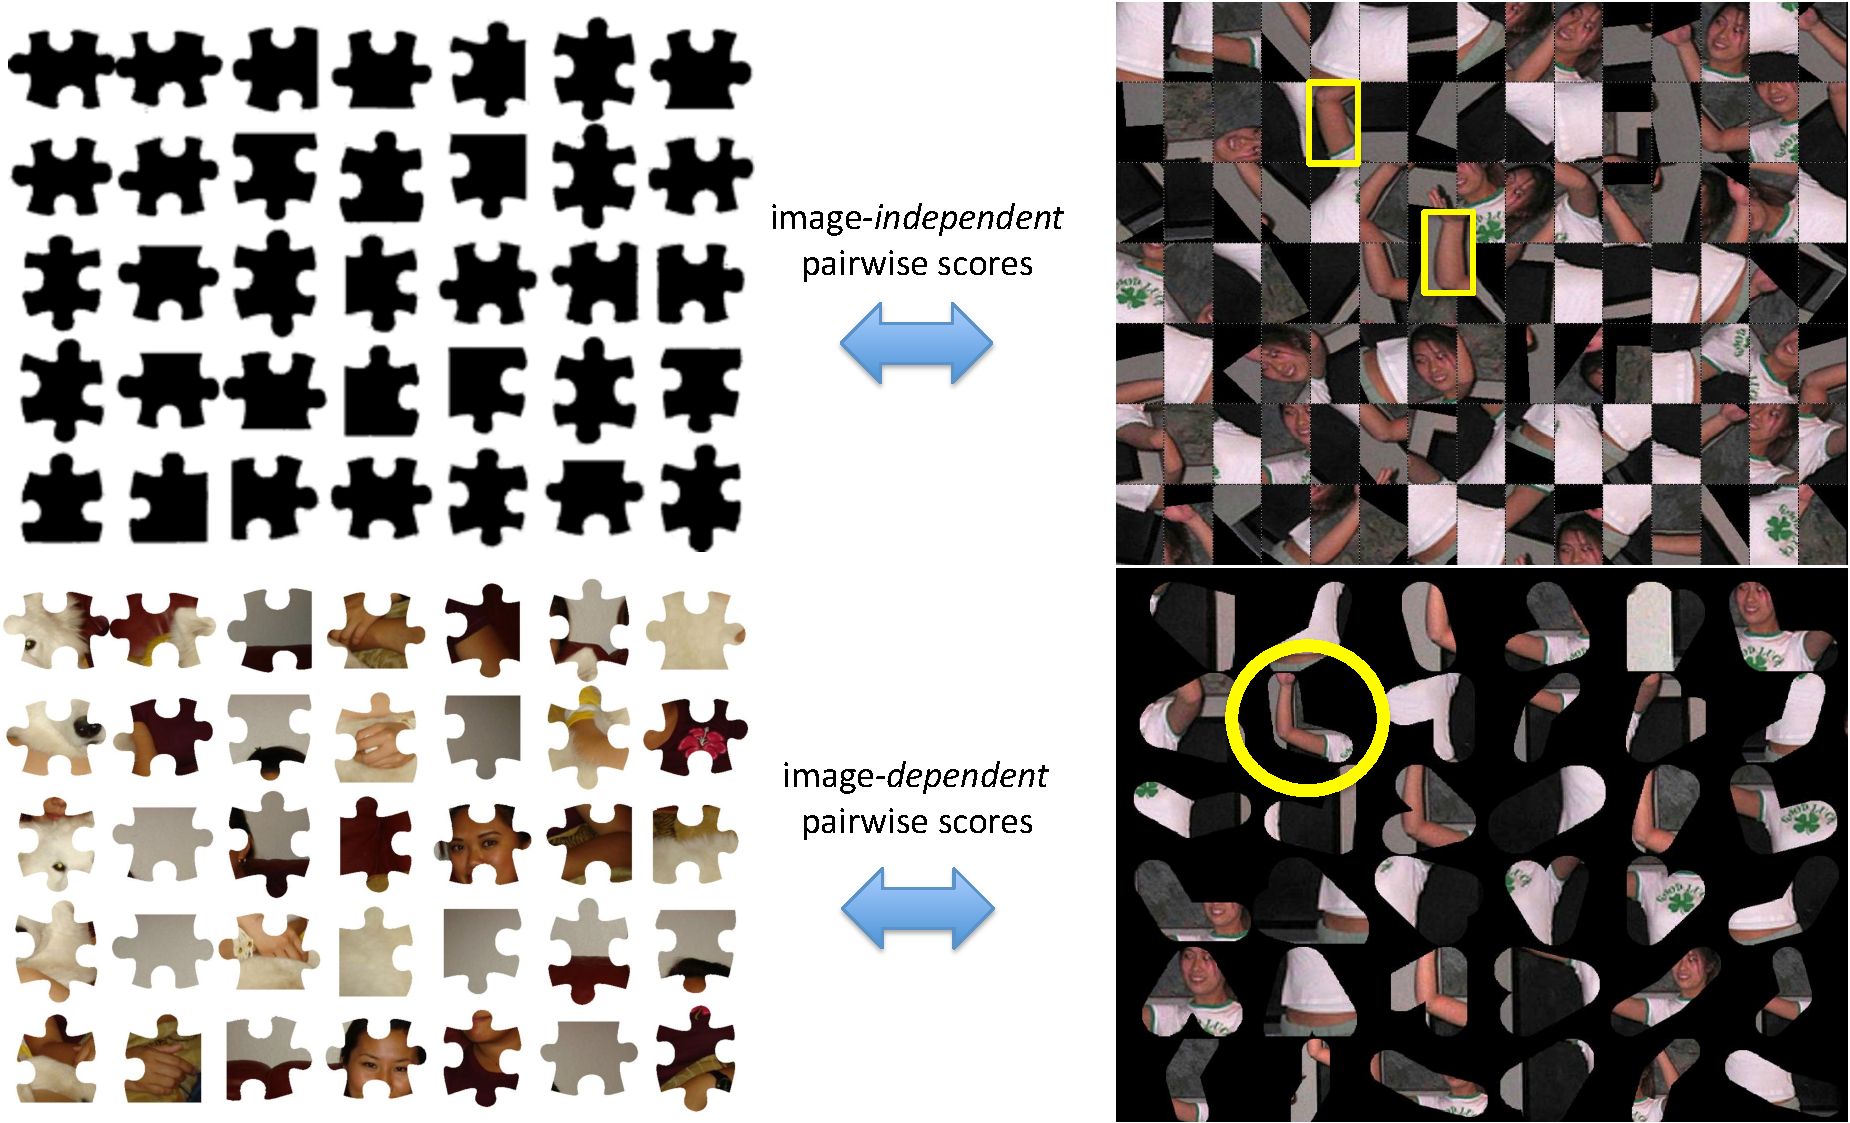
\includegraphics[width=0.99\textwidth]{figs/puzzle.pdf}
\caption[Puzzle analogy of pose estimation.]{Puzzle analogy of pose estimation.  
Classical approaches only use individual part detectors and geometric 
plausibility to determine the pose of a person.  This is analogous to 
attempting to put together a puzzle without looking at appearance of the pieces 
---only the plausibility of them fitting together. On the other hand, models 
with data-dependent interactions are analogous to using the appearance of the 
puzzle piece faces as well as their fit when constructing the puzzle.  Even for 
humans, it is easier to spot the correct pair of upper/lower arms when they are 
examined jointly.}
\label{fig:puzzle}
\end{center}
\end{figure}

Due to the computational issues discussed above, previous work in pose 
estimation has resorted to a model of pose that considers, at most, pairwise 
interactions between parts, in a specially restricted form: the network of 
part-pair interactions is described by a tree structured graph, and the 
interactions are described by simple kinematic consistency.  This is known as 
the basic {\em pictorial structure} (PS) model, also referred to as a {\em 
spring model}---see \secref{ps}, and \figref{spring-model-intro}.  

In PS models, each part has an individual score for placement at any location 
in the image, which must be balanced with part-pair penalties for deforming 
from the default model positions (``pose prior'').  For example, the 
deformation penalty between an upper arm and lower arm expresses the fact that 
they should roughly agree on where the elbow is.  The deformation penalties can 
be thought of as springs at rest at default positions and stretched by moving 
the parts to new positions.  The parts themselves are attracted individually to 
likely spots in the image.  Thus a balance is sought between individual part 
beliefs and respecting the prior notion of what a pose should look like.

\begin{figure}[tb]
\begin{center}
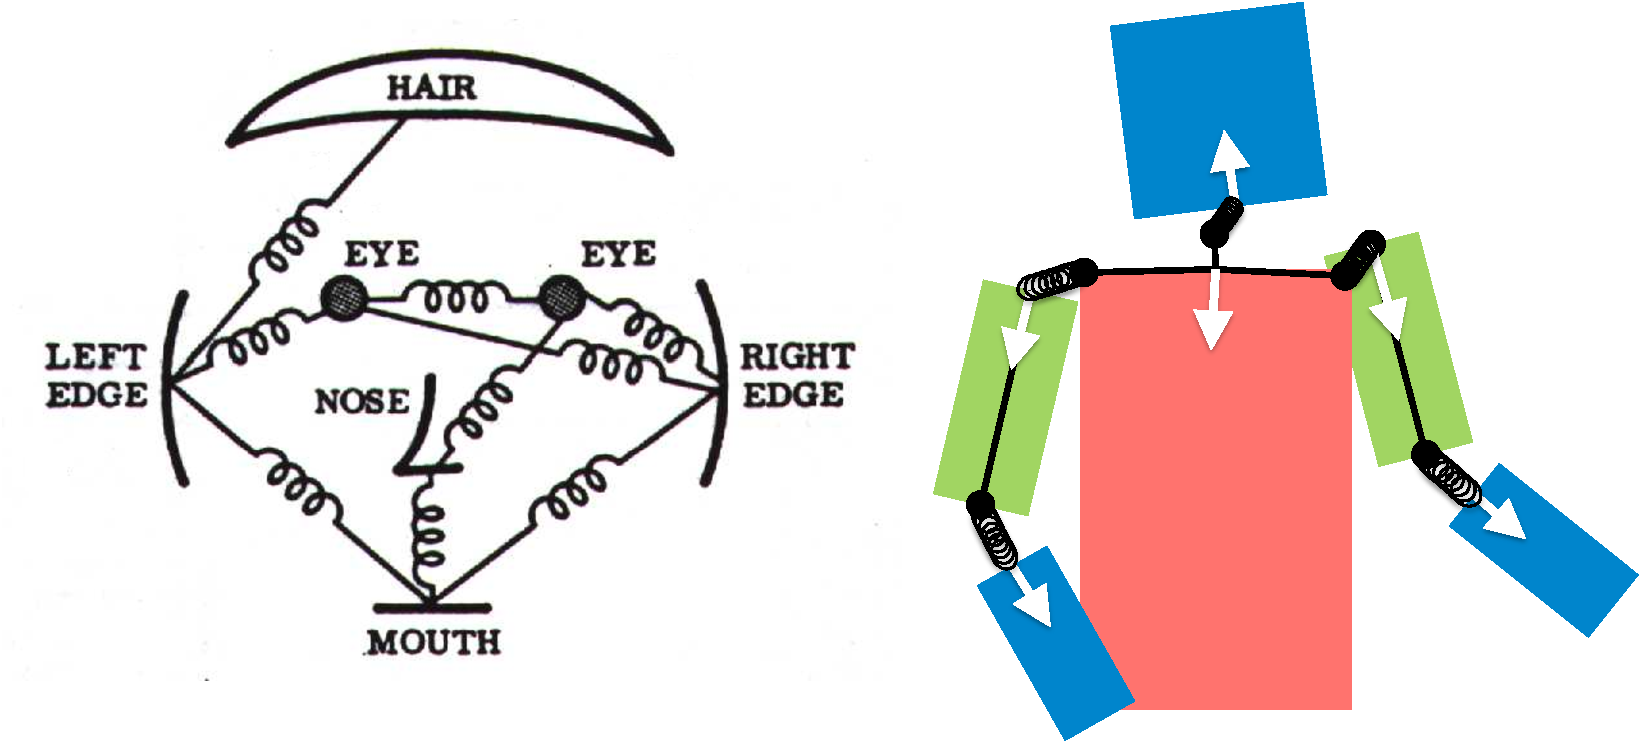
\includegraphics[width=0.99\textwidth]{figs/spring-model.pdf}
\caption[Spring model of pose.]{Spring model of pose.  At left, the original 
spring pictorial structure model that appeared in \citet{fischler1973ps}. At 
right, the standard PS model for 2D human pose.  The states are shown as unit 
vectors indicating the position of joints and their direction.  The mean 
displacement between joints are shown as solid black circles, connected by 
solid black lines to show the kinematic tree structure.  The displacement from 
mean positions are shown as springs stretching.  This figure is repeated again 
for convenience in \secref{ps}.}
\label{fig:spring-model-intro}
\end{center}
\end{figure}


An important property of PS models is that the pairwise, spring stretch, 
termsare {\em blind to the image content}.  The problem with this is that 
individual part detector scores are extremely weak (\secref{perceptual}): they 
must work in isolation and generalize to limbs in all settings of backgrounds, 
foregrounds, articulation, and environment.

As a result, the above model is effectively trying to piece together parts of a 
person, when the parts themselves are extremely ambiguous. As an extreme 
analogy of this, it is similar to attempting to put together a jigsaw puzzle in 
which the pieces themselves are very generic.  One has many plausible 
candidates for where each puzzle piece should go individually (like individual 
part scores), but to determine whether two pieces are adjacent, one can only 
see how well they fit together, and {\em not } the  image content on their 
faces; see \figreff{puzzle}{top row}.


\subsection{Image-dependent interactions in a tree structured 
model,~\secref{CPS}}
\label{sec:contrib1}
As an improvement over the basic PS model, we wish to actually {\em exploit } 
image content when modeling pairwise interactions.  In the puzzle analogy, this 
would allow us to fit pieces together based on their color similarity and 
continuous contours across the connection boundary; see \figreff{puzzle}{bottom 
row}.  We exploit these same cues for determining whether limbs go together in 
an image, as well as additional cues such as region support and multimodal 
descriptions of geometry.

Unfortunately, this turns out to be computationally infeasible using standard 
tools and techniques.  In light of this, we propose a {\em cascade} of models 
to focus computation on pose possibilities that are more promising.  There are 
many pose possibilities that are easy to reject as incorrect with a simple 
model (like a basic PS model, or even simpler), and we are then able to freely 
apply a richer model on the possibilities that remain.  This is illustrated 
in~\figref{cps-overview}.

To employ a cascade approach, we develop and analyze {\em structured prediction 
cascades}, and apply them to the problem of 2D pose estimation. Importantly, we 
provide a novel training objective for the cascade so that parameters of the 
models are learned to specifically to filter out a significant proportion of 
possibilities at every cascade level. 

\subsection{Image-dependent interactions in a general 
graph,~\secref{stretchable}}
The cascade approach we proposed in the previous section works for any 
tree-structured model.  However, in any tree model, we fail to capture 
important interactions between parts, both {\em within} a single frame (\eg, 
color constancy between left/right symmetric parts to model clothing) and {\em 
across} frames when dealing with tracking multiple parts and their interactions 
over time in video.  Determining the best possible answer $\argmax_y s(x,y)$ 
over a general cyclic graph of part relationships is known to be 
$\#P$-hard~\citep{koller-book}---exponential in the number of frames of video.  
We provide an approximate approach which decomposes a cyclic model of pose  
into a collection of subgraph trees, whose union of edges covers all the 
relationships we care to model.  This allows us to exploit all the interesting 
interaction terms in the original model with efficient inference in each 
subtree, thanks to the structure and the use of our cascade approach.
Then, we can exploit all cues used in the tree-based model, and in addition, 
cues based on color symmetry across the body, and temporal appearance and 
location persistence information.  We propose and investigate empirically 
different methods of reaching a consensus between the subtrees.

We evaluate our approach on a new video dataset, the first of its kind in 
tracking human pose in the wild without any assumed extra knowledge. We show 
our proposed model and approximation scheme is beneficial, beating the 
state-of-the-art in pose estimation systems.

\subsection{Multimodal interactions,~\secref{llps}}
\label{sec:contrib3}
The aforementioned models focus attention on increasing the quality of features 
and increasing the number of modeled part interactions.  The hope is that these 
more expressive models do a better job at capturing the inherently multimodal 
appearance space of poses, by better separating the true pose configurations 
from false alarms.  This somewhat addresses the issue of non-linearity in 
lower-dimensional feature spaces, \eg, using only edge information.

Complementary to the models described in the previous sections, we propose to 
capture this nonlinearity directly with an explicitly multimodal model.  Now 
the goal is to determine not only the best pose layout, but also which {\em 
mode} the pose belongs to.
Each mode need only model a portion of the pose space.  Instead of fitting the 
parameters of one monolithic model to cover all possible modes, here we learn 
separate parameters for each mode, allowing us to learn more precise 
descriptions of appearance and geometry, for, \eg, an arms crossed mode, an 
arms raised mode, etcetera. 

\subsection{Technical summary of models}

This section is intended for readers who already have an understanding of 
pairwise structured models and the parts-based pose estimation literature.  It 
provides a quick overview of the model formulations discussed in depth in the 
rest of this thesis.  It does not give a self-contained explanation, and the 
unfamiliar reader is encouraged to skip this section.

\begin{center}
\line(1,0){250}
\end{center}

\noindent The basic pictorial structure model takes the form $$ s(x,y) =  
\sum_{i \in \cV_{\tree}} \phi_i(x,y_i) + \sum_{i,j \in \cE_{\tree}} 
\phi_{ij}(y_i - y_j) $$
where the network of part pairwise interactions is described by a tree 
structured graph $\tree = (\cV_\tree,\cE_\tree)$.  The first terms 
$\phi_i(x,y_i)$ score how likely a part is to be placed at location $y_i$, 
independent of other parts.  The pairwise terms $\phi_{ij}(y_i-y_j)$ score the 
geometric compatibility between pairs of parts.  Importantly, this pairwise 
term is {\em blind to the image content}. 

Instead, we wish to actually {\em exploit } image content when modeling 
pairwise interactions. To this effect, in \secref{CPS} we propose a more 
general model of human pose, of the form \begin{equation}
\boxed{s(x,y) =  \sum_{i \in \cV_{\tree}} \phi_i(x,y_i) + \sum_{i,j \in 
\cE_{\tree}} \phi_{ij}(x,y_i,y_j)}
\label{eq:contrib1}
\end{equation}
This turns out to be computationally infeasible using standard tools and 
techniques.  We develop and analyze  structured prediction cascades as a tool 
to deal with this.  The cascade works by progressively filtering the state 
space of a sequence of models with coarse-to-fine resolution.  We pose a 
learning objective so that the models prune both aggressively and accurately at 
test time.


The model we propose \equref{contrib1} works for any tree-structured model, but 
cannot be applied to cyclic models.  We address this with a generalization 
of~\equref{contrib1}:
\begin{equation}
\boxed{s(x,y) =  \sum_{i \in \cV_{G}} \phi_i(x,y_i) + \sum_{i,j \in \cE_{G}} 
\phi_{ij}(x,y_i,y_j)}
\label{eq:contrib2}
\end{equation}
where $G = (\cV_G,\cE_G)$ is a general graph, not just a tree.  Determining the 
best possible answer $\argmax_y s(x,y)$ over a general graph $G$ is known to be 
$\#P$-hard~\citep{koller-book}---exponential in the number of frames of video.  
To deal with this, we explore state-of-the-art approximation techniques, such 
as dual decomposition, and propose a simpler approximation technique the 
performs at least as well with orders of magnitude less computation.  See 
\secref{stretchable}.

The aforementioned models focus attention on increasing the quality of features 
and increasing the number of modeled part interactions.  The hope is that these 
more expressive models do a better job at capturing the inherently multimodal 
appearance space of poses, by better separating the true pose configurations 
from false alarms.  This somewhat addresses the issue of non-linearity in 
lower-dimensional feature spaces, \eg, using only edge information.

Complementary to the models described by~\equref{contrib1} 
and~\equref{contrib2}, in \secref{llps} we propose to capture this nonlinearity 
directly as follows:
\begin{equation}
\boxed{s(x,y,z) =  \sum_{i \in \cV_{G}} \phi_i(x,y_i,z) + \sum_{i,j \in 
\cE_{G}} \phi_{ij}(x,y_i,y_j,z)}
\label{eq:contrib3}
\end{equation}
where now the goal is to determine not only the best pose layout $y$, but also 
which {\em mode} $z$ the pose belongs to: $y^\star,z^\star = \argmax_{y,z} 
s(x,y,z)$.  Each mode need only model a portion of the pose space.  Instead of 
fitting the parameters of one monolithic model to cover all possible modes, 
here we learn separate parameters for each mode, allowing us to learn more 
precise descriptions of appearance and geometry.



\subsection{Summary of contributions}

In summary, the work detailed in this thesis contributes the following to the 
fields of machine learning and computer vision, and especially their 
intersection for human pose estimation:
\begin{itemize}

\item New models of human pose that capture image-dependent interactions.

\item Computational innovations that enable learning and inference in these 
models, which are \naively intractable: structured cascades and tree ensemble 
methods.

\item A variety of new features and feature types not typically applied to pose 
estimation.  Some of these are bottom-up type features complementary to the 
traditional edge-based cues.

\item State-of-the-art results on the public Buffy and Pascal Stickmen single 
frame datasets, and our introduced MoviePose single frame and VideoPose video 
sequence datasets.

\end{itemize}


\subsection{Published work supporting this thesis}


The Cascaded Pictorial Structure model (\secref{CPS}) first appeared in 
\citet{sapp2010cascades} and introduced the concepts of a coarse-to-fine 
cascade that allows one to use arbitrary features efficiently.  This extended 
the original Structured Prediction Cascades approach from \citet{cascades}, 
with a journal version under review---\citet{cascades-jmlr}.
Using the cascade approach for an ensemble of models was developed in 
\citet{weisssapp10}.  This idea was then extended beyond cascade filtering for 
prediction in the Ensembles of Stretchable Models framework 
(\secref{stretchable}) for pose estimation in video in \citet{sapp2011}.  The 
complementary non-parametric approach of Local Linear Pictorial Structures 
(\secref{llps}) is currently to be submitted---\citet{sapp-llps}.


\clearpage
\part{Models and methods}
\chapter{Cascaded Pictorial Structures}\label{sec:CPS}


\section{Introduction}
Pictorial structure models, first proposed by ~\cite{fischler1973ps} and outline in~\secref{ps}, are a popular method for human body pose estimation~\cite{felz05,fergus2005sparse,devacrf,ferrari08,andriluka09}.
The model is a pairwise structured model over pose variables that characterizes 
local appearance properties of parts and geometric part-part interactions.   
The search over the full pose space is linear time in the number of parts when 
the part-part dependencies form a tree.  However,  the individual part 
state spaces are too large (typically hundreds of thousands of states) to allow 
complex appearance models to be evaluated densely.   Most appearance models are 
therefore simple linear filters on edges, color and 
location~\cite{felz05,devacrf,ferrari08,andriluka09}. 

Similarly, because of quadratic state-space complexity, part-part relationships 
are typically restricted to be image-independent deformation costs that allow 
for convolution or distance transform tricks to speed up 
inference~\cite{felz05}, see~\secref{ps}. A common problem in such models is 
poor localization of parts that have weak appearance cues or are easily 
confused with background clutter (accuracy for lower arms in human figures is 
almost half of that for torso or head~\cite{andriluka09}).   Localizing these 
elusive parts requires richer models of individual part shape and joint 
part-part appearance, including contour continuation and segmentation cues, 
which are prohibitive to compute densely.

In order to enable richer appearance models, we propose to learn a cascade of 
pictorial structures (\CPS) of increasing pose resolution which 
progressively filter the pose state space.  Conceptually, the idea is similar 
to the work on cascades for face detection~\cite{geman2001,viola02}, but the 
key difference is the use of structured models. Each level of the cascade works on a certain spatial and angular resolution.  A level refines the set of candidates from the 
previous level and then runs inference to determine which poses to filter out.  
For each part, the model selects poses with the largest {\em max-marginal}
scores, subject to a computational budget.  Unlike conventional pruning 
heuristics, where the possible part locations are identified using the output 
of a detector, models in our cascade use inference in simpler structured models 
to identify what to prune, taking into account global pose in filtering 
decisions.
\begin{figure}[t]
\begin{center}
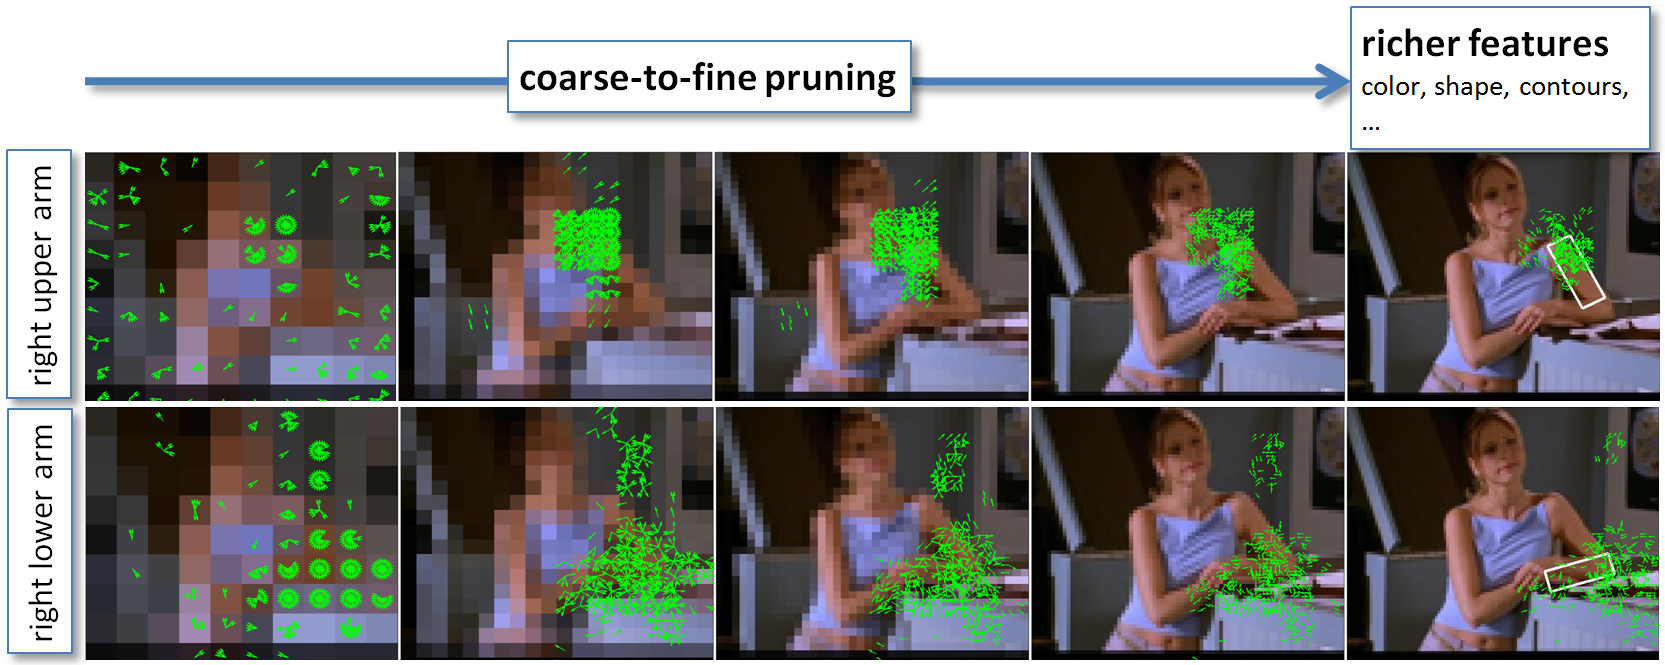
\includegraphics[width=1.0\textwidth]{figs/cps-overview.png}
\end{center}
\caption[Overview of Cascaded Pictorial Structures 
(CPS)]{\label{fig:cps-overview} Overview of CPS:  A discriminative 
coarse-to-fine cascade of pictorial structures filters the pose space so that 
expressive and computationally expensive cues can be used in the final 
pictorial structure.  Shown are 5 levels of our coarse-to-fine cascade for the 
right upper and lower arm parts.  Green vectors represent position and angle of 
unpruned states, the downsampled images correspond to the dimensions of the 
respective state space (but {\em not } the resolution at which features are 
computed), and the white rectangles represent classification using our final 
model.}
\end{figure}
As a result, at the final level the \CPS{} model has to deal with a much 
smaller hypothesis set which allows us to use a rich combination of features.  

In addition to the traditional part detectors and geometric features, we are 
able to incorporate object boundary continuity and smoothness, as well as shape 
features, discussed in detail in~\secref{features}. The former features 
represent mid-level and bottom-up cues, while the latter capture shape 
information, which is complementary to the traditional HoG-based part models.  
The approach is illustrated in the overview Figure~\ref{fig:cps-overview}. We 
apply the presented \CPS model combined with the richer set of features on the 
Buffy and PASCAL Stickmen benchmark, improving the state-of-the-art on arm 
localization, as discussed in~\secref{experiments}. 

\label{subsec:our_ps}
We choose instead to model part configurations as a general linear MRF over 
pairwise and unary terms:
\begin{align}
s(x,y)  = \w \cdot \f(x,y) = \sum_{i \in \cV_\tree} \w_i \cdot \f_i(x,y_i)  + 
\sum_{ij \in \cE_\tree} \w_{ij} \cdot \f_{ij}(x,y_i,y_j)
\label{eq:cps}
\end{align}
where $\tree = (\cV_\tree,\cE_\tree)$ defines a tree structured graph of part 
interactions.  The parameters of our model are the pairwise and unary weight 
vectors $\w_{ij}$ and $\w_i$ corresponding to the pairwise and unary feature 
vectors $\f_{ij}(x,y_i,y_j)$ and $\f_i(x,y_i)$.   The key differences with the 
classical PS model are (1) our pairwise costs allow data-dependent terms, and 
(2) we do not constrain our parameters to fit any parametric distribution such 
as a Gaussian distribution, as is done 
in~\citet{felz05,devacrf,andriluka09,eichner09}.  This is strictly more 
general.  For example, we can express the pairwise features used in the 
classical model as $y_{i} \cdot y_{i}$, $y_{j}\cdot y_{j}$, and $y_{i}\cdot 
y_{j}$ without requiring that their corresponding weights can be combined into 
a positive semi-definite covariance matrix.

In this general form (\equref{cps}), inference can {\em not} be performed 
efficiently with distance transforms as discussed 
in~\secref{dt}, and we rely on standard $O(nk^2)$ dynamic programming 
techniques to compute the best scoring assignment $\argmax_y s(x,y)$.  However, this remains efficient and sub-quadratic in practice through the use of cascades.

\section{Related work}
For unstructured, binary classification, cascades of classifiers have been 
quite successful for reducing computation.  \citet{geman2001} propose a 
coarse-to-fine sequence of binary tests to detect the presence and pose of 
objects in an image.  The learned sequence of tests is trained to minimize 
expected computational cost.  The extremely popular Viola-Jones 
classifier~\citep{viola02} implements a cascade of boosting ensembles, with 
earlier stages using fewer features to quickly reject large portions of the 
state space.

Our cascade model is inspired by these binary classification cascades. In 
natural language parsing, several works \citep{carreras2008tag,petrov:PhD} use 
a coarse-to-fine idea closely related to ours and~\citet{geman2001}: the 
marginals of a simple context free grammar or dependency model are used to 
prune the parse chart for a more complex grammar.

Recently,~\citet{pff-cascade} proposed a cascade for a structured parts-based 
model.  Their cascade works by early stopping while evaluating individual 
parts, if the combined part scores are less than fixed thresholds.  While the 
form of this cascade can be posed in our more general framework (a cascade of 
models with an increasing number of parts), we differ from~\citet{pff-cascade} 
in that our pruning is based on thresholds that adapt based on inference in 
each test example, and we explicitly learn parameters in order to prune safely 
and efficiently. In~\citet{geman2001,viola02,pff-cascade}, the focus is on 
preserving established levels of accuracy while increasing speed.  The focus in 
this paper is instead developing more complex models---previously infeasible 
due to the original intractable complexity---to improve state-of-the-art 
performance.

A different approach to reduce the intractable number of state hypotheses is to instead propose a small set of likely hypotheses based on bottom-up perceptual grouping principles~\cite{mori04,Srinivasan07}.  Mori et al.~\cite{mori04} use bottom-up saliency cues, for example strength of supporting contours, to generate limb hypotheses.  They then prune via hand-set rules based on part-pair geometry and color consistency. The shape, color and contour based features we use in our last cascade stage are inspired by such bottom-up processes.  However, our cascade is solely a sequence of discriminatively-trained top-down models.



\section{Structured Prediction Cascades} \label{sec:SPC}
The recently introduced Structured Prediction Cascade framework~\cite{cascades} 
provides a principled way to prune the state space of a structured prediction 
problem via a sequence of increasingly complex models.
There are many possible ways of defining a sequence of increasingly complex 
models.  In~\cite{cascades} the authors introduce higher-order cliques into 
their models in successive stages (first unary, then pairwise, ternary, etc.).  
Another option is to start with simple but computationally efficient features, 
and add more complex features downstream as the number of states decreases.  
Yet another option is to geometrically coarsen the original state space and 
successively prune and refine.
 We use a coarse-to-fine state space approach with simple features until we are 
at a reasonably fine enough state space resolution and left with few enough 
states that we can introduce more complex features.  We start with a severely 
coarsened state space and use standard pictorial structures unary detector 
scores and geometric features to perform quick exhaustive inference on the 
coarse state space.  

\subsection{Inference}
\begin{figure}[tb]
\begin{center}
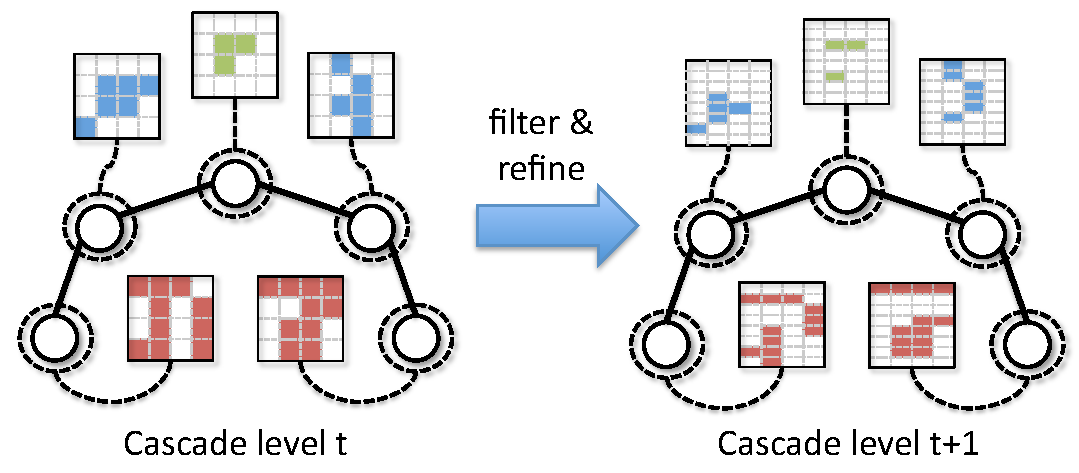
\includegraphics[width=0.99\textwidth]{figs/cascade-concept.pdf}
\caption[Intermediate cascade filtering/refinement step.]{Two consecutive stages of a cascade, showing a model with a sparse set of states in a coarsened state space (top) filtering out states, and then passing them on to the next model (bottom) which works on a finer, upsampled version of the state space.}
\label{fig:cascade-concept}
\end{center}
\end{figure}


The procedure for CPS described above is as follows.  Two intermediate steps of the process are conceptualized in~\figref{cascade-concept}.

\begin{itemize}
\item For an input $x$, initialize a coarse state space $\cS_0 = \cY_0$ by 
spatially pooling states in the original space (downsampling the original state space 
volume).

\item Repeat for each cascade level $t = 0,\ldots,T-1$:
\begin{itemize}
\item Run sparse, exact inference over  $\cS_t$ using the $t^{th}$ cascade 
model, computing max-marginal scores.
\item Filter states based on max-marginal scores to obtain $\tilde{\cS}_t$:\\
\indent For each $i$, filter $y_i$ if $\mmi < t_x$, a data-dependent threshold (see~\secref{cps-thresh}).

 \item Refine the state space of $\tilde{\cS}_t$ to obtain $\cS_t$ for 
the next cascaded model.
\end{itemize}
\item Predict using the final level: $y^\star = \argmax_{y \in \cY_T} s(x,y)$.
\end{itemize}


The key ingredient to the cascade framework is that states are pruned using 
{\em max-marginal} scores, introduced in~\secref{max-marginals}, computed 
efficiently using dynamic programming techniques.  The notion of a max-marginal 
is intuitively explained in our model of pose estimation:  The max-marginal for 
a part $i$ at location $y_i$ is the score of the highest scoring pose with part $i$ fixed or ``pinned'' to location $y_i$. Importantly, max-marginals are a {\em 
global} quantity of a complete model of pose, rather than a local one: A part 
could have weak individual image evidence of being at location $y_i$ but still 
have a high max-marginal score if the rest of the model believes this is a 
likely location for the part. 

\subsection{Filtering threshold}\label{sec:cps-thresh}

When applying a cascade, we have two competing objectives that we must trade 
off: accuracy and efficiency. We want to minimize the number of errors incurred 
by each level of the cascade  and maximize the number of filtered 
max-marginals.  A natural strategy is to prune away the lowest ranked states 
based on max-marginal scores. Instead, we prune the states whose max-marginal 
score is lower than a data-specific threshold $t_x$: $y_i$ is pruned if $\mmi < 
t_x$.  This threshold is defined as a convex combination of the highest score
$s^\star_x = \max_y s(x,y)$ and the {\em mean max-marginal score}, defined as:
\begin{equation}
\bar{s}^\star_x = \frac{1}{n} \sum_{i=1}^n \frac{1}{|\cY_i|} \sum_{y_i \in 
\cY_i} \mmi.
\end{equation}
which is just the average $\mmi$ over all parts and all states for each part.  Our thresholding function is thus
\begin{equation}
t_x(s,\alpha) = \alpha s^\star_x + (1-\alpha)\bar{s}^\star_x
\end{equation}
where $\alpha\in[0,1]$ is a parameter to be chosen that 
determines how aggressively to prune. When $\alpha = 1$, only the best state is 
kept, which is equivalent to finding the best, unconstrained assignment.  When $\alpha = 0$ 
approximately half of the states are pruned (if the median of max-marginals is 
equal to the mean).  The reasons for choosing this particular form of $t_x(s,\alpha)$ are (1) it is a 
function of the image $x$, which allows a threshold that adapts to the 
difficulty of the problem, and (2) it leads to a convex learning formulation 
with additional guarantees, as opposed to sorting max-marginals and choosing a 
cutoff.

\out{
The advantage of using  $t_x(s,\alpha)$ is that it 
is convex in $s(x,y)$, and leads to a convex formulation for parameter 
estimation that trades off the proportion of incorrectly pruned states with the 
proportion of unpruned states.
Note that  $\alpha$ controls efficiency, so we focus on learning the parameters $\theta$ that 
minimize the number of errors for a given filtering level $\alpha$.   
}
\subsection{Learning}
The goal of learning is to fit parameters to our models $\w$ such that they are 
optimized for the task of filtering states efficiently and accurately.  This is 
notably different than standard supervised learning, which attempts to find 
$\w$ to separate the right answer from wrong.  In some sense, the filtering 
learning object is easier to learn---the correct answer does not have to be the 
highest scoring, but only above the threshold value.  To wit, we pose the 
following hard-constraint learning objective, assuming a training set of pairs 
$\{(x^{(j)},y^{(j)})\}_{j=1}^M$:
\begin{align}
\minimize_\w& \frac{1}{2} ||\w||_2^2 \\
\subjectto& s(x^{(j)},y^{(j)}) \geq t_{x^{(j)}}(s,\alpha) + 1,\;\;\; \forall \; j
\end{align}
In words, the above is attempting to find a regularized set of weights $\w$ 
such that, in every training example, the score of the correct pose is above 
our image-adaptive threshold.  We convert the hard constraint objective into an 
unconstrained hinge-loss form typical of a max-margin structured learning 
problem (see~\secref{learning}):
\begin{align}
\minimize_\w& \frac{\lambda}{2} ||\w||_2^2 + \frac{1}{M} \sum_{j=1}^M \left[ 
t_{x^{(j)}}(s,\alpha) - s(x^{(j)},y^{(j)}) + 1 \right]_+
\label{eq:cps-learn-hinge}
\end{align}


The learning formulation uses a simple fact about max-marginals and the 
definition of $t_x(s,\alpha)$
to get a handle on errors of the cascade:
if $s(x,y) > t_x(s,\alpha)$, then for all $i$, $\mmi >  t_x(s,\alpha)$, so no 
part state of $y$ is pruned.   Given an example $(x,y)$,
this condition $s(x,y) > t_x(s,\alpha)$ is {\em sufficient} to ensure that no 
correct part is pruned, which is our justification for using max-marginals as 
the pruning quality.  Note that probabilistic marginals do {\em not} have this 
property: $p(y|x)$ being above a threshold does not guarantee that $p(y_i|x)$ 
are above a threshold for all $i$.

We solve \eqref{eq:cps-learn-hinge} using stochastic
subgradient descent. Given an example $(x,y)$, we apply the following when the 
term $\left[ t_x(s,\alpha) - s(x,y) + 1 \right]_+$ (and the subgradient) is 
non-zero:
\begin{equation} \label{eq:spf_update}
\w  \leftarrow \w + \eta \left[-\lambda \w + \f(y,x) - \alpha \f(y^\star,x)  - 
(1-\alpha) \bar{\f}^\star(x) \right].
\end{equation}
Above, $\eta$ is a learning rate parameter, $y^\star = \argmax_{y'}
s(x,y')$ is the highest scoring assignment and $\bar{\f}^\star(x)$ are the 
average features used by all max-marginal witnesses $\witnessi $ (explained 
in~\secref{max-marginals}):
\begin{equation}
\bar{\f}^\star(x) = \frac{1}{n} \sum_{i=1}^n \frac{1}{|\cY_i|} \sum_{y_i \in 
\cY_i} \f(x,\witnessi).
\end{equation}
The key distinguishing feature of this update as compared to
structured perceptron is the last term which subtracts features included in all
max-marginal assignments $\witnessi$.

\out{\footnote{Note that because \eqref{eq:convex_opt} is $\lambda$-strongly 
convex,
if we chose $\eta_t = 1/(\lambda t)$ and add a projection step to keep 
$\theta$ in a closed set, the update would correspond to the Pegasos
update with convergence guarantees of $\tilde{O}(1/\epsilon)$ iterations for
$\epsilon$-accurate solutions~\cite{shalev-shwartz07pegasos}.  In our experiments, we found the projection step made no difference and used only 2 passes over the data, with $\eta$ fixed.}.
%, as we discuss in Section~\ref{implementation}.
}

\mypar{Sequential cascade learning} The stages of the cascade are learned 
sequentially, from coarse to fine, and each has a different set of parameters 
$\w$ and $\mathcal{Y}_i$ for each part, as well as $\alpha$.  The states of the 
next level are simply refined versions of the states that have not been pruned.  
We describe the refinement structure of the cascade in~\secref{experiments}.

\out{
In the end of a coarse-to-fine cascade we are left with a small, sparse set of 
states that typically contains the groundtruth states or states relatively 
close to them---in practice we are left with around 500 states per part, and 
95\% of the time we retain a state the is close enough to be considered a match 
(see Table~\ref{tab:pruning}). At this point we have the freedom to add a 
variety of complex unary and pairwise part interaction features involving 
geometry, appearance, and compatibility with perceptual grouping principles 
which we describe in Section~\ref{sec:features}.
}

\subsection{Why not just detector-based pruning?} A \naive approach used in a 
variety of applications is to simply subsample states by thresholding outputs 
of part or sparse feature detectors, possibly combined with non-max 
suppression.  Our approach, based on pruning on max-marginal values in a 
first-order model, is more sophisticated: for articulated parts-based models, 
strong evidence from other parts can keep a part which has weak individual 
evidence, and would be pruned using only detection scores.  The failure of 
pre-filtering  part locations in human pose estimation is also noted 
by~\citet{andriluka09}, and serves as the primary justification for their use 
of the dense classical PS.  This is illustrated in~\figref{cascade-pruning}.

\begin{figure}[tb]
\begin{center}
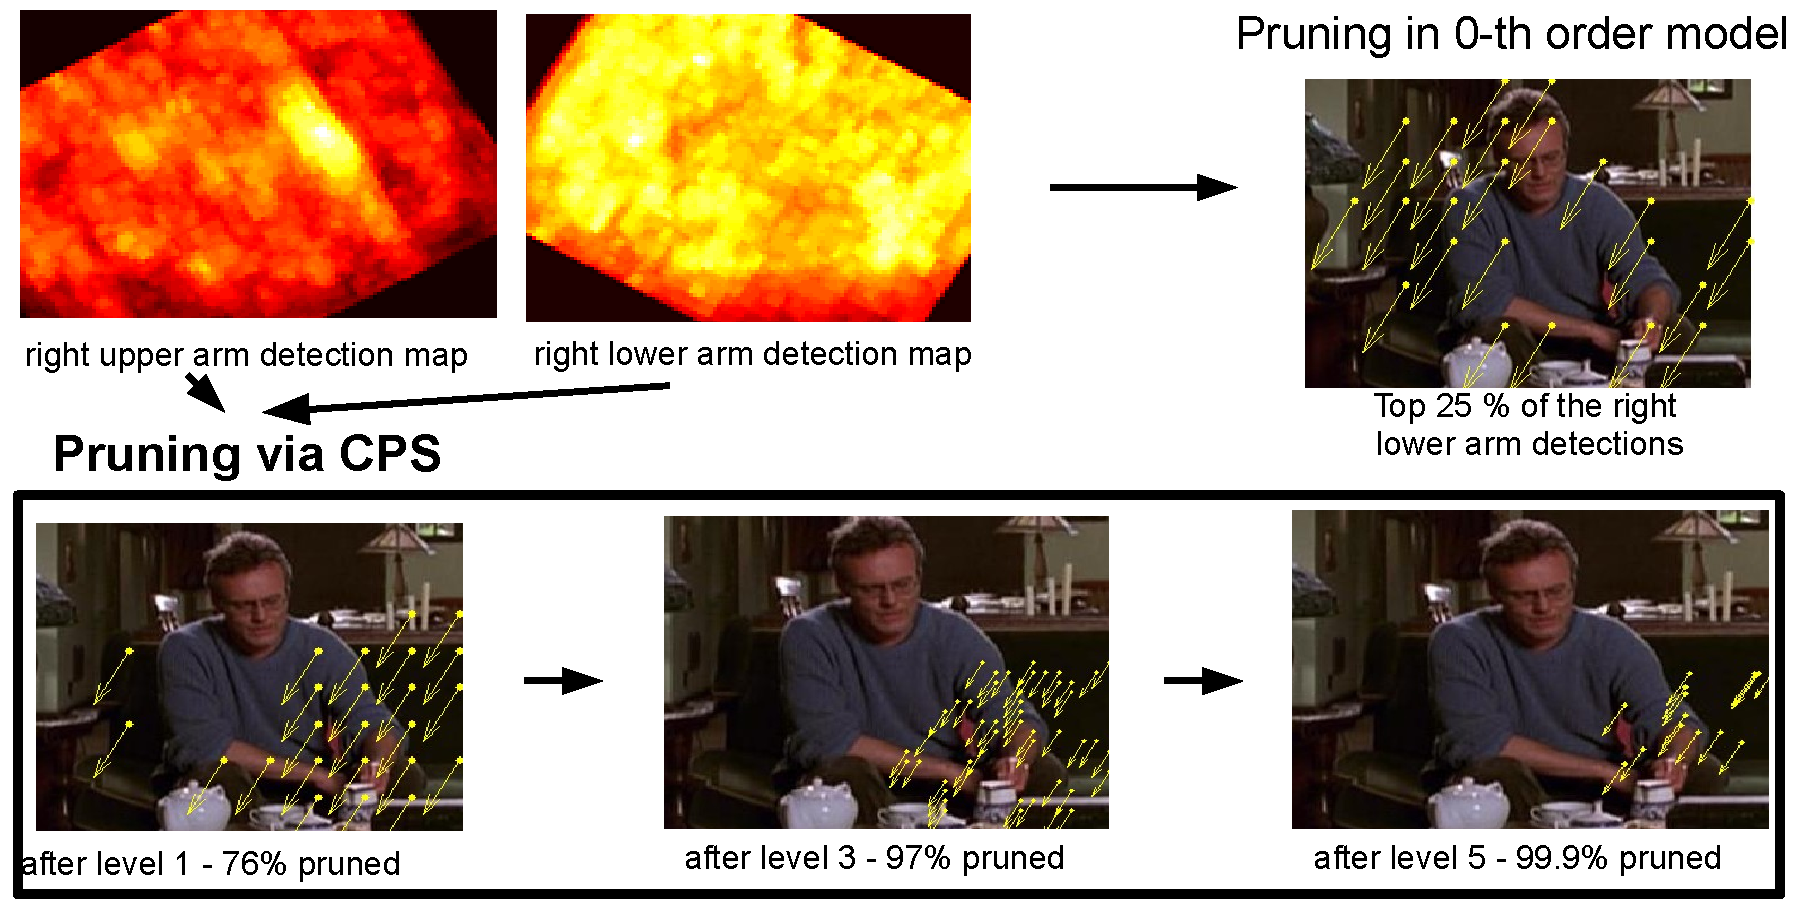
\includegraphics[width=0.99\textwidth]{figs/cascade-pruning.pdf}
\caption[Cascade filtering example]{Cascade filtering example. Detector-based 
pruning ($0^{th}$-order model) by thresholding yields many hypotheses far way from 
the true one for the lower right arm. The CPS (bottom row), however, exploits 
global information (such as certainty in the shoulder location) to perform 
better state pruning.}
\label{fig:cascade-pruning}
\end{center}
\end{figure}





\chapter{Ensembles}


\begin{figure}[t!]
\centering

\includegraphics[width=0.99\linewidth]{figs/empty.jpg}
\caption{\small \label{fig:overview} Overview. On the left, we show a full model with edges representing all pairwise relationships we want to capture within and between frames.  We approximate this full, intractable loopy model by decomposing it into an ensemble of six models which cover the edge relationships of the full model.  Our joint-centric representation is considerably more flexible in modeling pose variability than rigid limb-based representations~\cite{ferrari08,sapp2010cascades,andriluka09}.}
\label{fig:overview}
\end{figure}


% What we mean by motion parsing: articulated pose estimation + tracking = articulated motion parsing
We focus on the task of estimating and tracking articulated 2D human pose in videos ``in the wild'': single-view, uncontrolled settings typical in movies, television and amateur video.   Reliable
parsing of human motion in such videos could vastly improve and refine action 
recognition and semantic retrieval. This task is made difficult by the 
considerable background clutter, camera movement, motion blur, poor contrast, 
body pose and shape variation, as well as illumination, clothing and appearance 
diversity. There has been an explosion of recent work on articulated pose 
estimation from single images of this type~\cite{ronfard02, 
miko04,felzps,ramanan06,ferrari08,eichner09, andriluka09,sapp2010cascades}.  
Despite steady advances, localization of the most interesting parts (lower arms 
and hands) remains very inaccurate.  Video provides additional motion cues, yet 
most work on articulated tracking requires manual initialization from a few
frames~\cite{cardboard02,bregler98,balan06,sminchisescu03,ren07,buehler08}.  
Several recent papers~\cite{sigal04, lan05,ramanan05,ferrari08,weisssapp10}, 
however, combine tracking and estimation without any supervised initialization; 
our work follows this setting, which we call {\em articulated motion parsing}.

% Intractability, loopy, sampling, etc..
In the ``strike-a-pose'' parsing method of~\cite{ramanan05}, an easily 
detectable canonical pose (e.g., limbs spread out) is automatically found in a 
long stretch of video and used as initialization for person-specific part 
appearance models.  While this intuitive idea works well when every person 
strikes the easy canonical pose at least once in every video, many motion 
sequences are short and all the poses are difficult.  Most work to date on 
short, difficult motions does not show significant improvement over single 
frame parsing~\cite{ferrari08,weisssapp10}, and sometimes causes actual 
degradation in accuracy when pose estimation is coupled across frames.
One crucial reason for this is that joint parsing of multiple articulated parts over time involves  intractable inference and learning problems, since part location/orientation variables have very large state spaces and the models are highly inter-connected  (high-treewidth). Because of this barrier, previous work has resorted to approximate inference using sampling~\cite{wang07,isard98,sminchisescu03,sigal04} and variational~\cite{sigal2004tracking,ferrari08} methods, which often introduce poorly understood error and/or bias.
The computational complexity of learning such models often limits the ability 
to learn rich features, resulting in using only simple, image-independent 
location-persistence coupling~\cite{ferrari08}.  %BT: Note that sigal04  actually has nice features.
One notable contrast to this is the work of~\cite{ren07}, which uses powerful 
image cues and inference to establish correspondences between frames and within 
frames.  However, their method makes greedy decisions  as it proceeds through 
frames in order to handle the intractability of maintaining a distribution of 
beliefs throughout the video sequence, and hence has no way of recovering from 
bad choices in earlier frames.

%(they also are concerned with tracking only single objects).

Computational considerations also usually lead to restrictive simplifying assumptions on geometry: 2D limb lengths are 
fixed (given global scale)~\cite{ramanan05,ferrari08,eichner09, andriluka09}.  
In typical video sequences this assumption is 
almost always violated because of foreshortening and body type variation, 
especially for the lower arms. For this paper, we collected a new challenging video dataset which extends the one in~\cite{weisssapp10}, which we call VideoPose2.0.  In VideoPose2.0, roughly 30\% of all lower arms are significantly foreshortened;  see Figure~\ref{fig:dataset} for a summary of the dataset variability.

In this work, we overcome these computational and modeling limitations
using an ensemble of tractable submodels which couple
locations of body joints within and across frames using rich
image-dependent cues.  We address the problems of foreshortening and
part scale variation by using joint centers (shoulders, elbows,
wrists) as parts~\cite{lee06,urtasun08,rogez08}, instead of
limbs. Each submodel in the ensemble tracks a
single joint through time (e.g., left elbow), and also models the
spatial arrangement of all joints in a single frame.  Because of the
tree structure of each submodel, we can perform efficient exact
inference and use rich temporal features that depend on image
appearance, e.g., color tracking and optical flow contours. The models
are trained discriminatively using a large-margin loss, and we
experiment with a range of inference techniques that introduce
increasing coupling between models (and thus increasing computational
cost). Intriguingly, we find that a highly efficient method of
enforcing agreement on single variables that we introduced in
\cite{weisssapp10} outperforms costly approximate inference using dual
decomposition.

\begin{figure}[tb!]
\centering

\includegraphics[width=0.9\linewidth]{figs/empty.jpg}
\caption{\small \label{fig:dataset} A summary of our new video dataset, VideoPose2.0. 
\textbf{Left:} A scatter plot of groundtruth joints (green dot = shoulder, blue 
circle = elbow, red square = wrist). \textbf{Right:} Histogram of lower arm 
lengths in our dataset, illustrating how important it is to model relative part 
length in a real world setting.  }
\end{figure}

%jointly using a simple but effective 
%relaxation that results in linear scaling in complexity with the number of 
%parts.  

Our earlier work~\cite{weisssapp10} first investigated an ensemble of models 
for tracking body parts, but with several key differences: the model is 
designed to simply prune away unlikely hypotheses for torso and shoulder
locations, whereas in this work we focus on predicting the location of 
shoulders, elbows and hands---a significantly harder task.  Furthermore, like 
other previous work, \cite{weisssapp10} shows only a small improvement over 
single-frame parsing, and likewise the only temporal cue used is geometric persistence.


%We use dual decomposition~\cite{bertsekas99,komodakis2007dualdecomp} for 
%decoding, which returns optimal integral solutions X\% of the time.  

We apply our motion parsing model on a new video dataset of highly varied and 
articulated poses from TV shows containing over 1,200 frames.  We show 
significant quantitative and qualitative improvements over state-of-the-art 
single-frame pose estimation approaches (in particular, wrist and elbow 
accuracy improves by greater than 15\%).  In summary, the novel contributions 
of this work are: \textbf{(1)} an efficient ensemble of tree models for parsing 
human motion which covers a complex set of pairwise relationships and includes 
rich, image-dependent features; \textbf{(2)} stretchable 2D layout models, as 
opposed to the rigid parts typically used in pose estimation;
\textbf{(3)} significant improvement over single frame parsing results 
(arguably a first in this setting) \textbf{(4)} a challenging new video dataset, VideoPose2.0, 
with a high degree of motion pose variability which shows limitations of 
state-of-the-art methods.  The VideoPose2.0 dataset, code and videos are available at 
\textit{http://vision.grasp.upenn.edu/video}.



\section{Modeling}\label{sec:model}
As discussed, due to the intractability of jointly tracking multiple objects through time, previous 
work has made limiting assumptions in both the representation of pose (i.e., 
the inability to model foreshortening or fine angular granularity), and the 
interactions between parts, which do not capture rich, image-dependent 
relationships.  We address each of these issues in a principled framework.

\subsection{Stretchable models of human pose}  One of the biggest limitations 
of current models of human pose is the ``cardboard people'' 
assumption~\cite{cardboard02}: that body parts are rigid patches of fixed size 
(up to a global scale).  In the Pictorial Structures (PS) framework~\cite{felzps}, the human is represented as a collection of parts with fixed lengths, 
which along with the position and angle of each joint, completely determines 
the pose of the person~\footnote{The seminal work of Felzenswalb et 
al.~\cite{felzps} uses 10 discretized scales per part, 
but all modern implementations of PS use one fixed scale~\cite{sapp2010cascades,ferrari08,andriluka09}, partly due to its prohibitive 
increase in the state space.}.  Thus, wrists are always a fixed distance away 
from elbows in these models. This is a frequently violated assumption in 
realistic video, due to foreshortening and variation in body type.  In the VideoPose2.0 dataset we  
introduce (Section~\ref{sec:experiments}), 30\% of lower arms 
are significantly foreshortened.

\mypar{Two joints $>$ one limb:} Rather than model human limbs as a position 
and orientation, we propose a model {\em directly on the pixel coordinates of 
each joint}.  Although this choice introduces more variables 
(one for each joint rather than for each part), the state space for each 
variable is drastically reduced because we no longer need to reason over a 
finely discretized set of angles in the state space, and we can now implicitly 
represent nearly any angle between parts.  In current PS implementations, this is a 
$24\times$ reduction in the state space of each variable.  In addition to 
this, because the length of the limb is now determined implicitly by the pixel 
distance between neighboring joints, the model naturally lends itself to 
capturing large variability in the part length.  Because of its ability to 
represent finely discretized limb length, we refer to this model as
{\em stretchable}, in contrast to the typical rigid, rectangle-based 
representation.

One side-effect of switching from a limb-centric to joint-centric model of 
pose is that unary attributes of the limb-centric model are now pairwise 
attributes of a joint-centric model.  Furthermore, pairwise attributes in a 
limb-centric model correspond to ternary attributes in a joint-centric model, 
which we do not use.  However, in a standard PS model, pairwise attributes are 
only image-independent functions of geometry, whereas in our model, pairwise 
potentials all incorporate image information, giving us overall a more 
expressive model than standard PS. 



\subsection{Structured Ensemble of Stretchable Models}
Ideally we want a model of human motion which captures important
relationships between all correlated parts.  This includes parts that
are connected kinematically (e.g., left elbow, left wrist), parts that
are left/right symmetric (e.g., left elbow, right elbow), and
instantiations of the same part in consecutive frames (e.g., left
elbow at time $t$, left elbow at time $t+1$).  Clearly, modeling all
these relationships together leads to cyclic dependencies
within a single frame (due to the three symmetry edges) and
between consecutive frames (due to the six tracking edges); see Figure~\ref{fig:overview}, left. 

However, in general, it is always possible to express the score of a
given state assignment in a full, intractable model as the sum of
scores under a set of tree sub-models that collectively cover every
edge in the full model. This is the key insight that allows us to
include all the rich relationships we desire: we {\em decompose} our
model of all interesting relationships related to parsing human motion
into an ensemble of submodels, all of which are trees (and therefore
tractable). Each tree submodel is responsible for tracking a single
joint through time and additionally models the corresponding set of
pairwise interactions between joints in a single frame
(Figure~\ref{fig:overview}, right).

\subsection{Formulation}
Formally, we pose this problem as a structured prediction task, where
the input $x$ is a video sequence of $\ell$ images and the output $y$ is a
sequence of $P\ell$ variables, where $P$ is the number of parts (joint
locations) included in the model. Each output $y_i$ is the 2-D
coordinate of some part joint (defined in a $80 \times 80$
discretization of the pixel space) in some frame.  We also use the shortcut notation 
$y_{\bf t} = \{ y_i \;|\; y_i \text{ is in frame } t \}$
to index all $P$ joint variables in frame $t$. Given a training set
$S = \{(x^{(j)},y^{(j)})\}_{j=1}^n$ of samples from a joint
distribution, the standard supervised learning task is to learn a
hypothesis $h: X \mapsto Y$ that minimizes the expected loss $\E{S}{
  \cL\left(h(x^{(j)}) , y^{(j)}\right)}$ for some non-negative loss function $\cL
: Y \times Y \rightarrow \reals^+$. The linear hypothesis class we
consider is of the form $h(x) = \argmax_y \score{y}$, where the
scoring function $\score{y} \triangleq \w \cdot \f(x,y)$ is the
inner product of a vector of parameters $\theta$ and a feature
function $\bft: X \times Y \mapsto \reals^d$ mapping $(x,y)$ pairs to
$d$ real-valued features. Let $G = (\cV,\cE)$ be our full graphical
pose model; we further assume that $\bft$ decomposes over the vertices
$\cV$ and edges $\cE$, so that
\begin{equation}
  \label{eq:model-score}
  \score{y} = \sum_{(i,j) \in \cE}\\w \cdot \f_{ij}(x,y_i,y_j) +
  \sum_{i \in \cV}\w \cdot \f_i(x,y_i).
\end{equation}
Note that edges $(i,j)$ may connect variables between consecutive
frames. Let there be $M$ tree sub-models, and $G_m = (\cV, \cE_m)$ be the sub-graph of $G$ corresponding
to the $m$'th one as in Figure~\ref{fig:overview}, right.  Then
we decompose the score $\score{y}$ into the sum of the scores of the
$M$ constituent sub-models: $\score{y} = \sum_{m=1}^M \pscore{y}$, the
score of the $m$'th model is as in Equation~\ref{eq:model-score}, restricted to the
edges $\cE_m$, i.e. $\pscore{y} =
\sum_{(i,j)\in\cE_m}\theta_m^\top\bft_{ij}(x,y_i,y_j) +
\sum_{i\in\cV}\theta_m^\top\bft_i(x,y_i)$. Note that we do not couple
parameters across different models $\theta_m$.

\out{
\begin{figure}[]
\centering

\includegraphics[width=0.9\linewidth]{figs/empty.jpg}
\caption{\small \label{fig:dd} Decoding with Dual Decomposition
  (examples). \textbf{Left:} The argmax predictions of each of the
  sub-models in the ensemble; note the disparity in predictions.
  \textbf{Right:} The prediction after running Dual Decomposition for
  500 iterations or until convergence (Yellow) compared to the
  predictions from \cite{sapp2010cascades} (Magenta).}
\end{figure}
}

\subsection{Structured Model Inference}
We explore several methods for combining the $M$ independent models
during test time to make a single final decision.  The methods form a
hierarchy of agreement criteria between the submodels: at one extreme,
we enforce the constraint that all submodels must agree on the
maximizing assignment to all variables, and at the other, inference is
completely decoupled across submodels. Note that there is an inherent
trade-off between the degree of agreement imposed on the models and the
computational cost of the corresponding inference.  We present our
inference methods by order of decreasing agreement below.

\paragraph{Full Agreement via Dual Decomposition.} A natural goal is
to find the argmax decoding of joint locations throughout the entire
sequence of frames using our original model in
Eq.~\ref{eq:model-score}. However, solving the argmax decoding problem
exactly is prohibitively expensive, due to the high treewidth of this
cyclic graph. We use the method of Dual Decomposition (DD)
\cite{bertsekas99,komodakis2007dualdecomp} to solve a linear
programming relaxation of the decoding problem as follows. Observe
that the argmax decoding problem of our full model can be decomposed
into $M$ sub-problems { if those problems are coupled through a global
  equality constraint}:
\begin{align}
  \label{eq:dual-decomp}
&\argmax_{y, y^1,\dots,y^m} \sum_{m=1}^M \pscore{y^m}  \textrm{ s.t. } \:  y^m=y  \quad{}\quad{(DD)}
\end{align}
Although the optimization \eqref{eq:dual-decomp} is still intractable because of the integral constraints, optimizing the {\em dual} of \eqref{eq:dual-decomp} is always
tractable (if we first drop the integrality requirement), but no longer guaranteed to return an optimal integral solution. We solve the dual problem with sub-gradient descent. Once complete agreement between all
$y^m$ is reached, then inference has converged to the exact solution
of \eqref{eq:dual-decomp} (although eventual convergence is not
guaranteed.) In our experiments, if dual decomposition did not
converge (after 500 iterations in practice, each requiring inference in all $M$ models), we used the maximum scoring primal variables found during
any descent iteration.

\out{To
solve the dual problem with sub-gradient descent, we introduce
Lagrange multipliers $\nu_{ik}^p$ for every possible state assignment
$y_i = k$ in every part model. We then alternate between updating the
dual variables $\nu^p$ and the primal variables $y^p$:
\begin{align}
  y^p & \leftarrow \argmax_y \left( \pscore{y} +  \sum_{i,k} \nu^p_{ik} \ind{y_i=k^p}\right) \\
  \nu^p_{ik} & \leftarrow \nu_{ik} - \alpha\left(  \ind{y_i^p=k} - \frac{1}{P}\sum_p \ind{y_i^p=k} \right),
\end{align}
where $\ind{\cdot}$ is the indicator function and $\alpha$ is a rate
parameter chosen according to the scheme given in
\cite{komodakis2007dualdecomp}.
} 


\paragraph{Single Frame Agreement.} An alternative to computing the
MAP decoding of the entire sequence is to find the argmax solution
while constraining model agreement to only a subset of the variables
at a time.  If we restrict our attention to the variables in a single
time frame only, inference is considerably simpler.  For each frame
$t$, we solve
\begin{equation}
\argmax_{y_{\bf{t}}'} \sum_{m=1}^M \max_{y : y_{\bf{t}} = y_{\bf{t}}'} \pscore{y} \quad{}\quad{(SF)}
\end{equation}
to obtain the joint configuration for that frame (remember $y_{\bf t}$
denotes the {\em set} of P joint variables in frame $t$).  In words,
the inner maximization finds the highest scoring sequence $y$ subject to
the constraint that the variables in frame $t$ are fixed at positions
$y_{\bf t}'$.  The outer argmax is over all possibilities of single
frame configurations $y_{\bf t}'$.  This extends the notion of a
max-marginal of a variable (see ~\cite{weiss10}) to a max-marginal
over {\em a set} of variables.  This method requires first computing
the max-product messages sent to variables in frame $t$, in each of
the submodels.  Finding the argmax decoding of $y_{\bf t}$ is then
equivalent to inference in a grid with P variables (in our case $P=6$
joints).  This can be solved exactly by forming cliques of size 3, for
which the message passing clique-tree forms a chain.  In each clique,
there are at most pairwise potentials, and since the state space of
each part is relatively small ($|Y_p| \leq 500$), the $O(\sum_p
|Y_p|^3)$ cost of this inference takes less than a second per frame in
practice, and in our experiments took about as long as performing inference in all $M$ tree submodels (i.e., twice as slow overall).


\paragraph{Single Variable Agreement.} 

We can further narrow our subset of interest down to a single variable
at a time \cite{weisssapp10}.  This is a weaker criteria for model
agreement, but yields cheaper and simpler inference.  This gives us
the following inference problem for the $i^{th}$ variable:
\begin{equation}
\argmax_{y_i'} \sum_{m=1}^M \max_{y: y_i=y_i'}\pscore{y} \quad{}\quad{(SV)}
\end{equation}
This can be solved by computing max-marginals for each model using standard forward-backward message passing, summing the $M$ max-marginal scores, and taking the highest scoring sum.
Note that this is actually equal to MAP decoding in the full model when  
all sub-models agree on the argmax, which rarely occurs in practice. However, in \cite{weisssapp10} we showed
empirically that this decoding is a useful approximation
of the full MAP decoding prediction. 

We also compared the above methods to predicting each joint using the single model in
the ensemble that incorporated temporal dependencies for that
specific part, which we call the $Independent$ decoding scheme.


\subsection{Learning} Although we enforce agreement during ensemble inference 
at {\em test time}, coupling inference during training for more than one 
variable is prohibitively expensive to use as part of a learning procedure.  
Thus we learn
parameters $\theta_m$ using {\em decoupled} inference separately for
each model. To learn parameters, we optimize a convex hinge-loss
objective for each model separately. Let $\pscoremaxj~=~\max_y~\pscorej{y}$ and $y^{\star(j)}$ a corresponding maximizer, then the learning problem is 
{\small
\begin{align*}
\min_{\theta_m} \frac{\lambda}{2}||\theta_m||^2 +
\frac{1}{n}\sum_{j=1}^n \left[ \pscoremaxj + \Ind{y^{\star(j)} \neq y^{(j)}} - \pscorej{y^{(j)}}  \right]_+
\end{align*}}
where $[\cdot]_+ = \max(0,\cdot)$.
\out{
$\theta_m^\star =
\min_{\theta_m} \frac{\lambda}{2} ||\theta_m||^2 +
\frac{1}{n}\sum_{i=1}^n H(x^{(i)},y^{(i)},\theta_m)$, where $H$ is the hinge loss function, 
$H(x^{(i)},y^{(i)},\theta_m) = \left[ \pscorei{y^{i}} - \max_y \pscorei{y} - \ind{y\ne y^{(i)}} \right]_+$.
}
We optimize
this problem via stochastic sub-gradient descent, and we choose
$\lambda$ and the number of training epochs using a held-out
development set to minimize error.




\chapter{Locally-linear pictorial structures}\label{sec:llps}
\section{Introduction}
\out{
Human pose estimation from single, 2D images holds great potential to assist in 
a wide range of applications---semantic indexing of images and videos, action 
recognition, activity analysis, and human computer interaction, to name a few.
However, human pose estimation ``in the wild'' is an extremely challenging 
problem.  It shares all of the difficulties of object detection, such as 
confounding background clutter, lighting, viewpoint, and scale, in addition to
significant difficulties unique to human poses.  }


In this chapter, we focus explicitly on the multi-modal aspect of the 2D pose 
estimation problem.  As discussed in~\secref{perceptual}, there is an enormous 
variation in foreground and background color and texture, and even given 
viewpoint and pose, the shape of body parts is highly variable due to clothing, 
relative scale variations, and articulation (causing foreshortening, 
self-occlusion and physically different body contours).

\begin{figure}[t!]
\centering
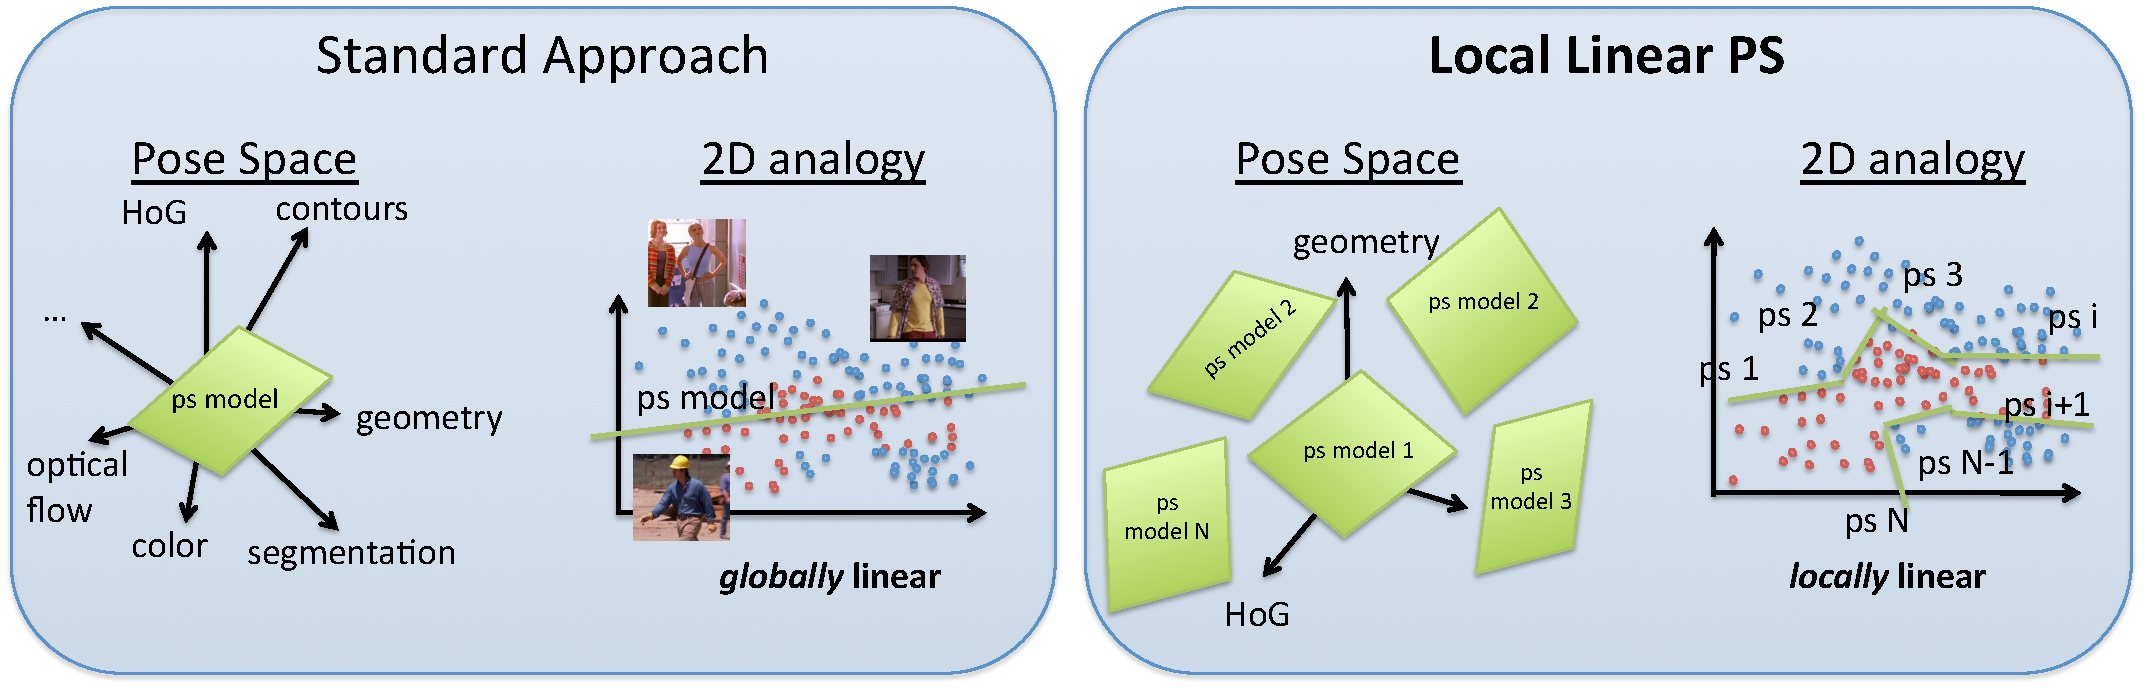
\includegraphics[width=0.99\linewidth]{figs/llps-overview.pdf}
\caption[LLPS overview.]{\label{fig:overview} \textbf{Left:} Most pictorial 
structures researchers have put effort into better and larger feature spaces, 
in which they fit one linear model.  The feature computation is expensive, and 
we still fail at capturing the many appearance modes in real data.  
\textbf{Right:} We take a different approach.  Rather than introduce more and 
more features in hopes of high-dimensional linear separability, we model the 
non-linearities in simpler, lower dimensional feature spaces, using a 
collection of {\em locally} linear models.}
\end{figure}


As a motivating example, consider the multitude of variations of left elbows, 
ignoring color and lighting variations.  First, there are a range of body 
types, yielding infant elbows and adult elbows, male elbows and female elbows, 
fat elbows and skinny---a conservative estimate would say there are 5 coarse 
body type modes.  Considering clothing, there are baggy long sleeves, tight 
long sleeves, stripes, solids, bare arms, and short sleeves ending near the 
elbow---let's assume we can summarize clothing variation around elbows with 5 
appearance modes (also overly optimistic).  Finally, given body type and 
clothing, we still must consider articulation.  A typical discretization of 
angles to model human pose~\citep{felz05,devacrf,eichner09} uses $15^\circ$ 
increments for a total of 24 possible relative angles.  As a rough 
back-of-the-envelope calculation, this already amounts to $5 \times 5 \times 24 
= 600$ major appearance modes, just for the elbow.  See~\figref{lelbs} for an 
illustration.


Clearly, some degree of sharing between appearance modes is warranted and 
beneficial, in particular because it is easier to estimate fewer model 
parameters.  However, most models developed for this problem take sharing to an 
extreme, and use {\em just a single, linear model}---\eg, 
\citet{devacrf,eichner09,andriluka09,ddtran} and the models developed 
in~\secref{CPS} and~\secref{stretchable}.
Such models make it very difficult to capture the part variations discussed.  
Most researchers focus attention on improving features in hopes that a better 
feature space will make a linear model fit well.  Only recently, several papers 
studied increasing the number of modes in pose models. However, these works 
used at most only tens of modes per part, and struggle with discovery of latent 
modes and/or defining an effective discrete quantization of the pose space.  
See \secref{llps-rel} for details.

\begin{figure}[tb!]
\centering
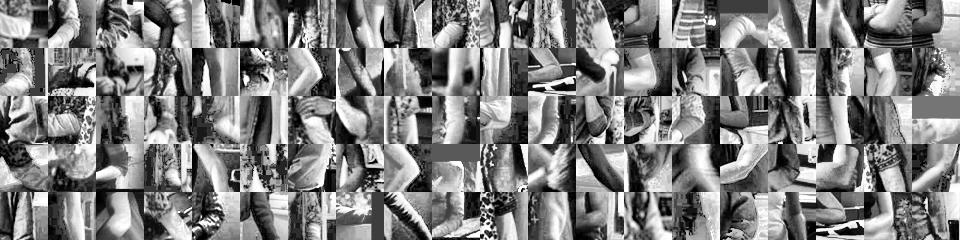
\includegraphics[width=0.99\linewidth]{figs/lelbs.jpg}
\caption[Elbow sample patches.]{ \label{fig:lelbs} A random sampling of 100 
left elbows from the Buffy Stickmen pose dataset, removing color and intensity 
bias, to illustrate the huge variety of appearance due to clutter, motion blur, 
clothing, body type, and pose.}
\end{figure}

\mypar{Our approach:} In this chapter, we propose a model of human pose that 
defines a mode {\em per training example}, to capture a local neighborhood of
pose {\em and } appearance.  This results in hundreds or thousands of modes in 
contrast to the 20 or fewer used by recent work. This gives us the ability to 
precisely model pose and appearance using a linear, structured model for each 
local neighborhood.  Because of this defining characteristic, we call our model 
\LLPSlong~(\LLPS).

We define the extent of each neighborhood in terms of radii in appearance and 
pose, which decompose at a part level.  As a result, the training example space 
is well covered, and we have overlap between modes.  This allows us to heavily 
share training data and gives us a smoothly varying representation of the space 
of 2D human poses.

Using our explicit formulation of locality, no latent modes need to estimated, 
and no decisions made as to quantization degree and mode placement.  We propose 
a simple convex max-margin learning objective to fit parameters of our model.  
We show our model is competitive with state-of-the-art approaches from this 
year, while employing only very simple features. Further, inference is cheap 
and heavily parallelizable, taking only a few seconds per image.


\section{Related work}
Here we take a particular perspective on some of the popular recent 
approaches~\citet{devacrf,eichner09,sapp2010cascades,sapp2011,andriluka09,ddtran}.  
Recently, there have been two major approaches to advance the performance of 
pictorial structures models:

\mypar{Throwing features at the problem:}  Equipped with a linear model of 
human pose, most researchers focus attention instead on increasing the quality 
of features, to be robust to the variety of modes discussed 
above---lighting-invariant texture modeling~\citep{andriluka09}, foreground and 
skin color~\citep{devacrf,eichner09}, left-right appearance 
similarity~\citep{ddtran,sapp2011}, contour and segmentation 
support~\citep{sapp2010cascades,sapp2011}, and more detailed description of 2D 
geometry~\citep{ddtran,sapp2011}, to name a few.  The hope in all of these 
models is that a linear model in a larger-dimensional feature space will be 
better able to separate the true pose configurations from false alarms, and 
mitigate the issue of non-linearity in lower-dimensional feature spaces, \eg, 
using only edge orientation information.

\mypar{Less features, more modes:} The cost of feature computation often 
dominates the computation time of pose estimation, \eg 
in~\citep{devacrf,sapp2010}.  Instead of attempting to add more and more 
features into one linear, additive model there has been a recent line of work 
that has begun to look at modeling multiple appearance modes.  Possibly the 
most famous example of this for rigid, non-articulated objects is the 
deformable parts model by Felzenszwalb et al.~\citep{dpm}, in which parameters 
for 6 different global modes (referred to as ``components'') are learned.  
Analogously in the pose estimation literature, Johnson and 
Everingham~\citep{johnson11} cluster training data based on joint locations into 
16 full-body modes, and learn a pictorial structures model separately for each.  
Increasing refinement, Yang and Ramanan~\citep{deva2011} introduced up to 5 
modes per part (referred to as part ``types'') in a pictorial structures model, 
allowing, \eg, 25 mode combinations for an elbow and wrist together.  Finally, 
Yang et al.~\citep{wang2011} proposed a hierarchical model of pose, in which 
each sub-pose is modeled with 5-20 modes (referred to as ``poselets'', inspired 
by~\citep{bourdev09}).

Of critical importance is how to choose modes to summarize the combined pose 
and appearance space of human bodies.  Having many modes gives a richer 
description and low intra-mode variability, but is difficult to estimate given 
finite training sets.  Having too few modes leads to high intra-mode 
variability and again leads to poor estimation via linear models. 

When a clear definition of a mode is not available, researchers have resorted 
to treating mode as a discrete latent variable to be estimated during 
learning~\citep{dpm,deva2011}.  This leads to non-convex optimization, in which 
careful initialization is important to avoid getting stuck in bad local minima.  
An alternative approach has been to define modes based on geometry, typically 
by clustering the space of joint locations into disjoint 
partitions~\citep{johnson11,wang2011}.  This has its own issues in choosing the 
right level of quantization, and how to cover the space of poses correctly.  
Importantly, {\em no} human pose estimation work considers defining modes as a 
function of appearance, which, as discussed, is the source of much of the 
nonlinearity in the space of 2D human poses. 

\mypar{Other local modeling methods:}
In the machine learning literature, there is a vast array of local methods for 
prediction.  Many of these require costly parameter estimation at test time, 
such as locally weighted logistic regression and KNN-SVM~\citep{zhang06}.  
Although we call our method locally linear, it does not estimate parameters at 
test time like these techniques.

Different from those, nearest-neighbor methods are powerful, but live and die 
by the right choice of distance function.  Standard norms fare poorly in 
high-dimensional spaces.  Learning distance functions for nearest neighbors has 
achieved some success, \eg Large-Margin KNN~\citep{lmknn}, which seeks to learn 
a global distance function for the whole sample space.  A refinement of this is 
to learn local distance functions---~\citep{frome07} and the recent 
Exemplar-SVM~\citep{esvm} both learn distance functions per example.  These 
works are quite similar in spirit to ours, but focus on object classification 
and detection, not structured, articulated part localization.

At the core of our method is a definition of a local neighborhood.  Our 
definition uses some of the same information used to define 
poselets~\citep{bourdev09}, which are clusters of subsets of pose 
configurations.  However, their model is a simple voting scheme for person 
detection.  There is no structure between parts (poselets), and no sharing or 
notion of overlapping neighborhoods.



\section{\LLPS}\label{sec:llps-model}

We pose the problem of 2D human pose estimation as a structured prediction 
task.  Let $x$ represent a given input image, and $y$ represent the location of 
$P$ parts in image coordinates.  Each variable $y_i$ denotes the pixel 
coordinates (row, column) of part $i$ in image $x$.  For ``parts'' we choose to 
model joints and their midpoints (\eg, left wrist, left forearm, left elbow) 
which allows us fine-grained encoding of foreshortening and rotation, as is 
done in~\citep{deva2011,sapp2011}.

The standard Pictorial Structures model described in~\secref{ps} is a linear 
model which decomposes into a sum of unary and pairwise linear terms.  We 
choose a general pairwise MRF form in which the score for a part configuration 
specified by $y$ in image $x$ is:
\begin{align}
 s(x,y) = \sum_{i \cV}^n \w_i \cdot \f_i(x,y_i) + \sum_{(i,j) \in \cE} \w_{ij} 
\cdot \f_{ij}(x,y_i,y_j),
 \label{eq:llps-ps}
\end{align}
When the graph $G = (\cV,\cE)$ describes a tree, we can use efficient dynamic 
programming techniques to infer the best scoring configuration of all parts 
(~\secref{inference}), $y^\star = \argmax_{y \in \mathcal{Y}} s(x,y)$.
The set $\mathcal{Y}$ denotes the entire set of possible poses, which is 
exponential in the number of model parts: $|\mathcal{Y}| = |\mathcal{Y}_i|^P$, 
where $\mathcal{Y}_i$ is the set of possible placements of part $i$ in the 
image (and is the same for all $i$).

% \subsection{\LLPSlong~(\LLPS)}
Instead of a single, linear model as in~\equref{llps-ps}, we model human pose 
with a collection of linear models which describe different local 
neighborhoods.  Let us consider $M$ such models, which we index $m = 1 \ldots 
M$:
\begin{align}
s^m(x,y) = \sum_{i=1}^n \w^m_i \cdot \f_i(x,y_i) + \sum_{(i,j) \in \mathcal{E}} 
\w^m_{ij} \cdot \f_{ij}(x,y_i,y_j),
\end{align}
Each model shares the same tree structure $\mathcal{E}$ and features 
$\f_i(\cdot),~\f_{ij}(\cdot)$ for the sake of simplicity; it is easy to extend 
this to a heterogenous collection of models.  The $M$ models' parameters $\w^M 
= [\w^m_i;~\w^m_{ij}]$ are learned to fit a local neighborhood around each 
training exemplar, discussed in~\secref{llps-learning}.

The full \LLPS model introduces an extra variable $z \in [1,M]$ into the state 
of the model to infer, at test time, both the best local model to use, and the 
best placement of joints given that model:
\begin{align}
s(x,y,z) &= s^z(x,y) \\
z^\star,y^\star &= \argmax_{z \in [1,M],~y \in \mathcal{Y}} s(x,y,z) 
\end{align}
Thus, given a test example, the test time inference procedure is 
straightforward (see~\figref{llps-inference}): evaluate all $M$ local models 
(in practice, up to thousands of them), via max-sum inference 
(\secref{inference}), saving the score and highest scoring output sequence of 
each.  Then, we take the highest scoring of the $M$ local models and its output 
sequence as a prediction of the pose.  This is transparently parallelizable and 
fits easily into popular parallelization frameworks, such as MapReduce.

\begin{figure}[tb!]
\centering
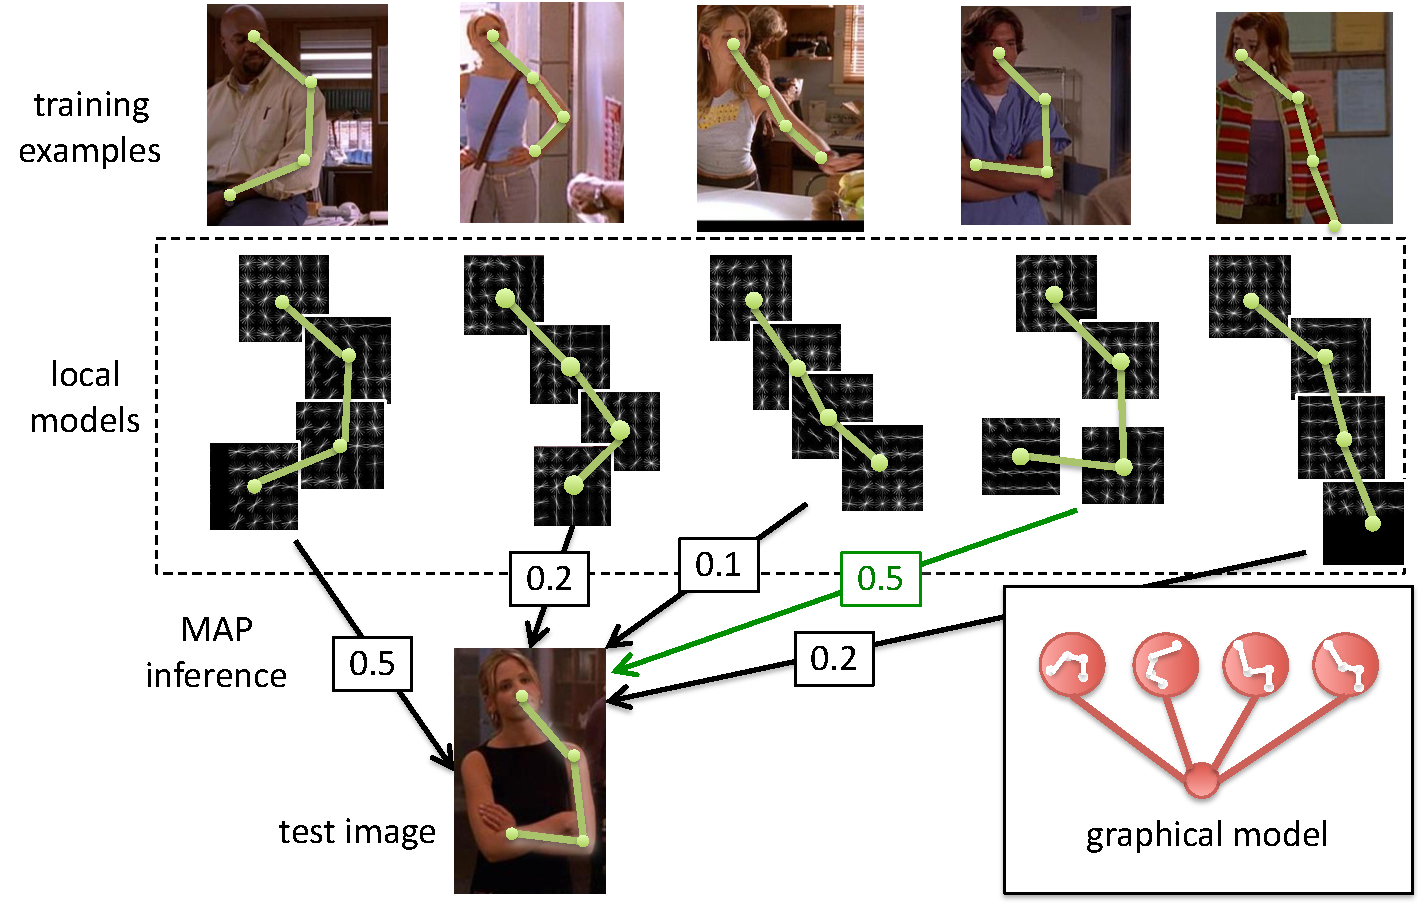
\includegraphics[width=0.99\linewidth]{figs/llps-inference.pdf}
\caption[LLPS inference.]{\label{fig:llps-inference} An illustration of the 
inference process.  Each training example defines a local neighborhood model.  
Each model is run in parallel on a test image, and the argmax prediction is 
taken as a guess. Inset: the graphical model structure.}
\end{figure}

\subsection{Image-adaptive pose priors and a non-parametric perspective}
One important perspective of the above is as a pose {\em switching model}, 
popular in speech synthesis \citep{rosti2003switching}.  In this setting, $z$ 
can be thought of as a switch which chooses between different appearance and 
pose priors.  The particular instantiation of $z$ depends on the image content.  
This is related to another, locally-linear method called Adaptive Pictorial 
Structures (APS) \citet{sapp2010}.  In this work, the pose prior terms 
$\phi_{ij}$ were adjusted based on a kernel-weighted sum of exemplar 
similarities to the image.  \LLPS, on the other hand, forces a discrete choice 
from a dictionary of pose priors, and this procedure is learned 
discriminatively.  From a more practical standpoint, APS relied on very costly 
and heuristic nearest-neighbor computation.  It searched densely through a 
large number of deformations to handle articulation, rather than making use of 
have a decomposable distance.  Each submodel of \LLPS can be thought of as a 
decomposable similarity function, learned discriminatively to separate true 
poses from bad locally, as we will see next.

\section{Learning}\label{sec:llps-learning}

During training, we have access to a training set of images with labeled poses 
$S = \{(x^{t},y^{t})\}_{t=1}^T$.  As described, we choose to model a local 
neighborhood in pose and appearance centered around each training example.  
This allows us to capture fine variations of appearance from pose, clothing, 
lighting, etcetera using a single linear model.

We define a neighborhood set function which maps an image and corresponding 
human pose to a set of indices of ``close'' training samples: $t \in 
\mathcal{N}((x,y))$ means that training sample $t$ is somehow ``close'' to 
$(x,y)$ in appearance and pose.  We will also overload notation to say the 
$\mathcal{N}(t)$ refers to the neighborhood of training sample $t$.  The 
specifics of $\mathcal{N}(\cdot)$ which formalize the notions of closeness in 
pose and appearance are detailed in \secref{nbhd}.

The key idea of learning is that we want to fit parameters so that each local 
model scores higher than other models that are not part of its local 
neighborhood, on the correct pose configuration.  For submodel $m$ centered 
about training sample $(x^m,y^m)$, we would like the large-margin constraints:
\begin{align}
s^m(x^t,y^t) \geq 1 + s^{m}(x^t,y), \label{eq:c1}\\
s^m(x^t,y^t) \geq 1 + s^{m'}(x^t,y),\label{eq:c2}\\
\forall y \in \mathcal{Y}\setminus \{y^t\},~\forall t \in 
\mathcal{N}(m),~\forall m' \notin \mathcal{N}(m) \nonumber
\end{align}
In words,~\equref{c1} states that the score of the true configuration for local 
model $m$ must be higher than $m$'s score for any other (wrong) configuration 
in example $t$.  \equref{c2} states that the score of the true configuration 
for $m$ must also be higher than any score a ``stranger'' model $m' \notin 
\mathcal{N}(m)$ has for any pose configuration in example $t$.  Adding slack 
and regularization on the parameters, we get a convex, large-margin structured 
loss jointly over all $m$ local models

\begin{align}\label{eq:full-learn}
\min_{\{w^m\}, \{\xi_{m,t}\}}& \;\; \sum_{m=1}^M ||w^m||_2^2 + C \sum_{m=1}^M 
\sum_{t \in \mathcal{N}(m)} \left[ \xi_{m,t} + \sum_{m' \notin \mathcal{N}(m)} 
\xi'_{m',t} \right] \\
\text{\bf{subject to:} }
&s^m(x^t,y^t) \geq 1 + s^{m}(x^t,y) - \xi_{m,t}\\
&s^m(x^t,y^t) \geq 1 + s^{m'}(x^t,y) - \xi'_{m',t}\\
&\forall y \in \mathcal{Y}\setminus \{y^t\}, \forall m \in [1,M], \forall t \in 
\mathcal{N}(m), \forall m' \notin \mathcal{N}(m) \nonumber \end{align}

Note that there is in practice significant overlap in neighborhood sets rather than disjoint partitions.  This gives a smoothly varying description of pose space.

\subsection{Decomposable approximate learning}
The learning objective in~\equref{full-learn} couples all models together to 
train them jointly.  While this has attractive properties, it is unwieldy for 
large training sets.  We now propose a series of modifications to the form of 
the model and~\equref{full-learn} to significantly simplify and parallelize 
training.

\mypar{A simpler pairwise cost:}\label{sec:boxdist}
Traditionally, the pairwise cost in PS models has been a simple geometric 
displacement cost: $f_{ij}(x,y_i,y_j) = d(y_i - y_j - \delta_{ij})$, where 
$\delta_{ij}$ is the mean pixel displacement vector between parts $i$ and $j$, 
and $d(\cdot)$ is either a quadratic penalty~\citep{felz05} or a binning 
function~\citep{devacrf}.  These restricted forms of $d(\cdot)$ allow for fast 
inference message passing techniques via convolution or distance transforms.  
We use instead a uniform {\em box deformation cost} defined by 
$f_{ij}(x,y_i,y_j) = 0$ when $|y_i - y_j - \delta_ij| < b$, and $-\infty$ 
otherwise, where $b$ specifies the size of the box in which, given $y_j$, $y_i$ 
is free to deviate from $\delta_{ij}$ in pixel units.  This yields a new form 
for our local model \begin{align}\label{eq:boxdist}
s^m(x,y) = 
\begin{cases}
 \sum_i \w^m_i \cdot \f_i(x,y_i), & |y_i - y_j - \delta_{ij}| < b,\;\; \forall 
(i,j) \in \mathcal{E} \\
 -\infty & \text{otherwise}
 \end{cases}
\end{align}

This formulation has attractive properties: (1) It leads to even faster inference than a quadratic stretching cost, using a 2D min transform instead of a distance transform, (2) less parameters to learn in each local neighborhood.

\mypar{Decoupling local models:} Next, we drop the constraints
$$s^m(x^t,y^t) \geq 1 + s^{m'}(x^t,y), \forall m, \forall m'\notin 
\mathcal{N}(m),\forall t$$ which decouples model $m$'s parameters from all 
other models $m'$.  Model $m$ no longer has to score the correct configuration 
$y^t$ higher than other models' beliefs in the correct configuration.  Instead, 
it only has to score the correct configuration higher than the exponentially 
many incorrect configurations in its local neighborhood of training images.  
This is equivalent to training a single PS model on a subset of the training 
data, independent of other models trained on other, overlapping subsets of the 
training data.  The inherent problem with this is that now different local 
model scores may not be comparable.  We address this with a calibration step 
described in~\secref{calib}.

\mypar{Psuedolikelihood} A final approximation is to assume, for training, that the structured functions $s^m(x,y)$ decompose into independent cliques, and can thus be trained independently.  That is,
$$ s^m(x,y) = \sum_{i} s^m(x,y_i | y_{\mathcal{E}(i)}) $$ 
where $\mathcal{E}(i) = \{j \;|\; (i,j) \in \mathcal{E}\}$.  This is a common 
trick that greatly simplifies structured learning, at the cost of approximation 
error.  Combined with the pairwise cost described in~\equref{boxdist}, this 
amounts to
$$s^m(x,y_i| y_{\mathcal{E}(i)}) = 
\begin{cases}
 \w^m_i \cdot \f_i(x,y_i), & |y_i - y_j - \delta_{ij}| < b,\;\; \forall j \in 
\mathcal{E}(i) \\
 -\infty & \text{otherwise}
\end{cases}
$$
which means we can learn parameters $\w_i^m$ separately for each part $i$ in 
each local model $m$.

In summary, by using a box deformation cost, decoupling the local models and using pseudolikelihood, we train part detectors individually.  The structured SVM learning objective for each part $i$ in each model $m$ is now:

\begin{align}
\min_{\w_i^m}&~||\w_i^m||_2^2 + C \sum_{t} \xi_t\\
\text{subject to: }
& \w_i^m \cdot \f_i(x^t,y_i^t) \geq 1+\w_i^m \cdot \f_i(x^t,y_i)-\xi_t 
\nonumber \\
& \w_i^m \cdot \f_i(x^t,y_i^t) \geq 1+\w_i^m \cdot \f_i(x^{t'},y_i)-\xi_t 
\nonumber \\
&\forall y_i \in \mathcal{Y}_i\setminus \{y_i^t\}, \forall t \in 
\mathcal{N}(m), \forall t' \notin \mathcal{N}(m) \nonumber
\end{align}
We can optimize this using an off-the-shelf standard binary SVM solver.  We 
handle the enormous number of constraints---$O(M \cdot |\mathcal{Y}_i|)$, the 
number of pixel locations in our dataset---by employing a cutting plane method, 
which starts from a random sampling of constraints, and iteratively finds 
violated constraints by mining for false positives, then re-optimizing.

	

\section{Modeling human pose with \LLPS}
In~\secref{llps-model} and~\secref{llps-learning}, we detailed a general 
learning and inference framework for local linear structured models, with 
overlapping and decomposable neighborhood structure.  We now fill in necessary 
details on the graph structure, neighborhood function, and features to describe 
how we apply this model to human pose estimation.
\subsection{Local graph structure}
In order to effectively use training data, we model only one side of a human--- 
the nose, left shoulder, left elbow and left wrist. This allows us to re-use 
training data for the left and right sides by horizontal mirroring, and also 
makes inference faster since we have a simple chain graph connecting each 
joint.  We also insert midpoint nodes into the graph between the semantic 
joints---between the nose and shoulder  (capturing neck curvature), the upper 
arm, and the forearm, similar to~\citet{deva2011}, and thus have $n=7$ parts in 
each local linear structured model.

The decision to split the modeling into sides is also justified empirically.  
Localization accuracy for detecting the torso and head of a person in pose
datasets is near-perfect, thus there is virtually no useful signal for the left 
side of a person to send to the right side through the torso and head, 
regarding beliefs of where parts should go.  In other words, variables on the 
left and right side of the person are d-separated given the torso and head 
variables, which are observed almost deterministically.

\subsection{Local Neighborhoods}\label{sec:nbhd}

As laid out in~\secref{llps-learning}, we define a neighborhood function 
$\mathcal{N}(x,y)$ which takes as input the appearance $x$ and human pose $y$ 
and returns a set of training example indices which are considered part of the 
neighborhood of example $(x,y)$.  We allow our neighborhood function to 
decompose at the level of parts, so that we can mix and match training examples 
when we train models for different joints.  For example, when learning 
parameters centered around example $t$, a different set of other examples may 
be used to train the elbow than are used to train the shoulder parameters.  We 
define our part-based neighborhood as follows, leveraging both appearance and 
geometry:

\mypar{Geometric neighborhood $\mathcal{N}_{geom}(y_i)$:} Around a joint $y_i$, 
we consider two angles and two limb lengths which we use to define our 
geometric neighborhood: the angle that limb $y_i$,$y_{i+1}$ makes with the 
horizontal axis, the inner angle between limbs $y_{i-1}$,$y_i$ and 
$y_{i}$,$y_{i+1}$, and the Euclidean length of limbs $y_{i-1}$,$y_i$ and 
$y_{i}$,$y_{i+1}$.  Stacking these $4$ geometric features into a vector $g_i$, 
we define our geometric neighborhood as $$ \mathcal{N}_{geom}(y_i) = \{\; t 
\text{ s.t. } |g_{ij} - g^t_{ij}| < \tau_j \text{ for $j=1...4$}\;\},$$ 
thresholding on differences of angles and limbs between the example center 
$y_i$ and all other examples $y_i^t$.  In practice we set $\tau_j$ to be a 
tolerance of $5^\circ$ for the two angles, and a tolerance of 6\% of the height 
of a detected upper body for the limb length (more intuitively, approximately 
the palm size of a human hand).


\mypar{Appearance neighborhood $\mathcal{N}_{app}(x,y_i)$:}  While there are 
many examples that are pose similar, we really wish to fit model parameters for 
a set of examples that {\em appears} similar, \eg, to avoid trying to model
different clothing or body types with one linear model.  In light of this, we 
consider a patch centered around joint $y_i$, represented as a HoG descriptor 
vector $h_i$.  We measure the similarity to other examples' HoG descriptor 
patches via normalized cross-correlation, and threshold to obtain our 
appearance neighborhood definition: $$  \mathcal{N}_{app}(x,y_i) = \{\; t 
\text{ s.t. } \frac{h_i}{||h_i||} \cdot \frac{h_i^t}{||h_i^t||} < \tau_h 
\;\},$$ where in practice we set $\tau_h = 0.2$ (normalized cross-correlation's 
range is $[-1,1]$).
Finally, we combine our appearance and geometry neighborhood definitions to 
obtain our neighborhood function $\mathcal{N}(x,y_i) = \mathcal{N}_{geom}(y_i) 
\cap \mathcal{N}_{app}(x,y_i).$

\subsection{Inter-Model Calibration}\label{sec:calib}  As described 
in~\secref{llps-learning}, we decouple the training of our local models, which 
allows us to efficiently train models in parallel.  The downside of this is 
that the bias and variance of the output of each model might vary greatly.  One 
very overconfident local model may always dominate the prediction step.  The 
problem of combining separately-trained models is also an issue in other recent 
works---\citet{johnson11} uses multinomial logistic regression on validation 
data to predict which of 16 PS models to believe per test example, and
Exemplar-SVM~\citep{esvm}, lacking validation data, estimates posterior 
probabilities from already-seen training data. In our implementation, we 
perform inference for each local model on every training example---this data 
was seen during pseudo-likelihood training, but not in full model inference.  
We then estimate a linear scale and offset to map the range of scores of each 
local model on the training set to $[0,1]$.  \\
\mypar{Mode selection:} In an additional step, we also remove redundant or 
malevolent models---ones whose addition to the set of local models hurts 
performance.  On training data, after calibration, we start with an empty set 
of models, and then iteratively greedily choose to add a new local model that 
increases the accuracy of the inlier set.  If we consider each local model as a 
basis, this is a form of basis pursuit.  In practice this results in a 
significantly smaller set of local models at test time, which speeds up 
inference. Details are in~\secref{experiments}.  



\clearpage
\part{Higher-order image features}
\chapter{Features}\label{sec:features}

\myquotation{Do not call me a computer vision engineer \ldots  I am a perceptual 
scientist!}{Yiannis Alimonous}


The introduced \CPS model allows us to capture appearance, geometry and shape information of parts and pairs of parts in the final level of the cascade---much richer than the standard geometric deformation costs and texture filters of previous PS models~\cite{felz05,devacrf,ferrari08,andriluka09}.  
%Table~\ref{feat_table} lists all features that we use and will describe in this section.  
Each part is modeled as a rectangle anchored at the part joint with the major axis defined as the line segment between the joints (see Figure~\ref{fig:ps}).  For training and evaluation, our datasets have been annotated only with this part axis.

%The side of a part is defined as the longer side of part rectangle.  
%Further, the major axis of a part is the line segment starting at the part joint parallel to the part side.

%In the following, we will use the support of each part $l_i$ in the image defined as a rectangle anchored at the part joint position position $(l_{ix}, l_{iy})$ and aligned with the part orientation $(l_{iu}, l_{iv})$  (see Fig.~\ref{fig:ps}). The dimensions $(h_i, w_i)$ of the support rectangle for each part are predefined, where the width is set $0.25$ of the length. The side of the part is defined as the longer side of the supporting rectangle. Further, the main axis of a part is the line segment starting at the part joint parallel to the part side.

\begin{figure}[t!]
\begin{center}

\includegraphics[width=0.9\textwidth]{figs/empty.jpg}
\caption{\label{cc_fig} Left: input image; Middle left: segmentation with segment boundaries and their touching points in red. 
%A long sequence of boundaries form a contour if the angle at each touching point is small.
Middle right: contour edges which support part $y_i$ and have normals which do not deviate from the part axis normal by more than $\omega$. 
%Small $\omega$ results in edges which are parallel and close to the part axis.
Right: first and second order moments of the region lying under the major part axis.}
\end{center}
\vskip -0.4in
\end{figure}
\mypar{Shape}
We express the shape of limbs via region and contour information. We use contour cues to capture the notion that limbs have a long smooth outline connecting and supporting both the upper and lower parts.  Region information is used to express coarse global shape properties of each limb, attempting to express the fact the limbs are often supported by a roughly rectangular collection of regions---the same notion that drives the bottom-up hypothesis generation in~\cite{mori04,Srinivasan07}.
% of segments A second shape feature captures the notion that arms tend to have the shape of rectangles.

\mypar{Shape/Contour} We detect long smooth contours from sequences of image segmentation boundaries obtained via NCut~\cite{cour05}.
%sequences of boundaries of image segments.
We define a graph whose nodes are all boundaries between segments with edges linking touching boundaries. Each contour is a path in this graph (see Fig.~\ref{cc_fig}, middle left). To reduce the number of possible paths, we restrict ourselves to all shortest paths. To quantify the smoothness of a contour, we compute an angle between each two touching segment boundaries\footnote{This angle is computed as the angle between the lines fitted to the segment boundary ends, defined as one third of the boundary. }. The smoothness of a contour is quantified as the maximum angle between boundaries along this contour. Finally, we find among all shortest paths those whose length exceeds $\ell_{\textrm{th}}$ pixels and whose smoothness is less then $s_{\textrm{th}}$ and denote them by $\{c_1,\dots c_m\}$.\footnote{We set $\ell_{\textrm{th}} = 60$ pixels, $s_{\textrm{th}} = 45^\circ$ resulting in $15$ to $30$ contours per image.}

% To define the above features, we extract segments using NCut \cite{cour05}. For the contour features, we extract long smooth contours, each defined as a sequence of linked segment boundaries, such that the transitions between boundaries are smooth (see Fig.~\ref{cc_fig}, middle left). To obtain such sequences, we define a graph, whose nodes are all boundaries between segments with edges linking touching boundaries. For each pair of segment boundaries, we compute the shortest path between them, which represents a contour in the image. We retain contours which are longer than $l_{\textrm{th}}$ pixels and are smooth. To quantify the smoothness of a contour, we compute an angle between each two touching segment boundaries. This can be done by fitting a line to the segment boundary end, defined as one third of the boundary, and compute the angle between the the boundary ends at the touching point.  The smoothness of a contour is quantified as the maximum angle between boundaries along this contour. We retain contours whose smoothness is less than $s_{\textrm{th}}$. In our implementation we use $30$ segments and set $l_{\textrm{th}} = 60$ pixels, $s_{\textrm{th}} = 45^\circ$, which results in $m$ contours per image $\{c_1,\dots c_m\}$ for $m$ usually between $15$ and $30$.

We can use the above contours to define features for each pair of lower and upper arms, which encode the notion that those two parts should share a long smooth contour, which is parallel and close to the part boundaries. For each arm part $l_i$ and a contour $c_k$ we can estimate the edges of $c_k$ which lie inside one of the halves of the supporting rectangle of $l_i$ and whose edge normals build an angle smaller than $\omega$ with the normal of the part axis (see Fig.~\ref{cc_fig}, right). We denote the number of those edges by $q_{ik}(\omega)$. Intuitively, a contour supports a limb if it is mostly parallel and enclosed in one of the limb sides, i.e.~the value $q_{ik}(\omega)$ is large for small angles $\omega$. A pair of arm limbs $l_i$, $l_j$ should have a high score if both parts are supported by a contour $c_k$, which can be expressed as the following two scores
\[
  \textrm{cc}_{ijk}^{(1)}(\omega, \omega') = \frac{1}{2}\left(\frac{q_{ik}(\omega)}{h_i} + \frac{q_{jk}(\omega')}{h_j}\right)\quad\textrm{and}\quad\textrm{cc}_{ijk}^{(2)}(\omega, \omega') = \min\left\{\frac{q_{ik}(\omega)}{h_i}, \frac{q_{jk}(\omega')}{h_j}\right\}
\]
where we normalize $q_{ik}$ by the length of the limb $h_i$ to ensure that the score is in $[0,1]$. The first score measures the overall support of the parts, while the second measures the minimum support. Hence, for $l_i$, $l_j$ we can find the highest score among all contours, which expresses the highest degree of support which this pair of arms can receive from any of the image contours:
\[
\textrm{cc}_{ij}^{(t)}(\omega, \omega') = \max_{k\in\{1, \dots , m\}}\textrm{cc}_{ijk}^{(t)}(\omega, \omega'), \quad\textrm{for} \quad t\in\{1,2\}
\]
By varying the angles $\omega$ and $\omega'$ in a set of admissible angles $\Omega$ defining parallelism between the part and the contour, we obtain $|\Omega|^2$ contour features\footnote{We set $\Omega=\{10^\circ, 20^\circ, 30^\circ\}$, which results in $18$ features for both scores.}.
% For the left limbs we use the right half of the supporting rectangle, viewed from the part joint, while for the right limbs we use the left half. This corresponds to the outer contour of each arm

\mypar{Shape/Region Moments} We compute the first and second order moments of 
the segments lying under the major part axis (see Fig.~\ref{cc_fig}, 
right)\footnote{We select segments which cover at least $25\%$ of the part 
axis.} to coarsely express shape of limb hypotheses as a collection of 
segments, $R_i$. To achieve rotation and translation invariance, we compute the 
moments in the part coordinate system.  We include convexity information 
$|conv(R_{i})|/|R_{i}|$, where $conv(\cdot)$ is the convex hull of a set of 
points, and $|R_{i}|$ is the number of points in the collection of segments.  
We also include the number of points on the convex hull, and the number of part 
axis points that pass through $R_{i}$ to express continuity along the part 
axis. 
 
 Note that contour feature is a pure bottom-up cue which does not capture the 
precise arm shape but encodes figural properties of the arm -- smoothness and 
continuity of its boundary. It is a mid-level cue related to a configuration of 
two parts. The part shape, however, encodes a more precise shape but only of a 
single part.
 
\mypar{Appearance/Texture} Following the edge-based representation used in 
\cite{latentsvm}, we model the appearance the body parts using Histogram of 
Gradient (HoG) descriptor.  For each of the 6 body parts -- head, torso, upper 
and lower arms -- we learn an individual Gentleboost classifier 
\cite{friedman00} on the HoG features using the Limbs Annotated in Movies 
Dataset\footnote{LAMDa is available at 
\textit{http://vision.grasp.upenn.edu/video}}.  %The output of the classifier 
is our first appearance feature.

\mypar{Appearance/Color}  As opposed to HoG, color drastically varies between people. We use the same assumptions as \cite{eichner09} and build color models assuming a fixed location for the head and torso at run-time for each image.  We train Adaboost classifiers using these pre-defined regions of positive and negative example pixels, represented as RGB, Lab, and HSV components.  For a particular image, a 5-round Adaboost ensemble~\cite{freund1997decision} is learned for each color model (head, torso) and reapplied to all the pixels in the image.  A similar technique is also used by~\cite{strikeapose} to incorporate color.  
%Face and torso can reveal information about skin and clothing color of all other parts.  
Features are computed as the mean score of each discrimintative color model on the pixels lying in the rectangle of the part.

% on positive examples drawn from fixed rectangles, which roughly localize the person torso and head, and negative examples drawn from the background of training images. We use the color channels in RGB, Lab and HSV spaces for each pixels as features. Then we can use those models on unknown part hypotheses from the same image -- head and torso reveal information about the skin and clothing color which are same for the arm clothing and hand color. For an arm hypothesis, the two color features $f_2, f_3$ are computed as the mean score of the pixels lying in the support of the part using both models. 

We use similarity of appearance between lower and upper arms as features for 
the pairwise potentials of \CPS. Precisely, we use the $\chi^2$ distance 
between the color histograms of the pixels lying in the part support.  The 
histograms are computed using minimum-variance quantization of the RGB color 
values of each image into $8$ colors.
% Precisely, we use two features, the first $f_4$ being the $\chi^2$ distance between the color histograms of the pixels lying in the part support. The histograms are computed using minimum-variance quantization of the RGB color values of each image into $8$ colors. The second feature $f_5$ is defined in terms of the spectral embedding obtained from NCuts segmentation \cite{cour05}. NCuts is defined in terms of a pixel affinity matrix which encodes color and intervening contour similarities (see~\cite{cour05} for details). The final segmentation is obtained through discretization of the top eigenvectors (we use the top $30$) of the affinity matrix. These vectors define for each pixel an embedding vector (in our case of dimension $30$) with the property that the vectors in this embedding space are clearly clustered according to the NCut segmentation criterion and the cues used in the affinity matrix. Thus, the mean embedding vector of all pixels in the support of a body part can be interpreted as an segmentation embedding vector of the part. FInally, the dot product of two such vectors representing two arm parts can be interpreted as similarity score, which is our last appearance feature $f_5$.

\mypar{Geometry} The body part configuration is encoded in two set of features. 
The location $(l_{ix}, l_{iy})$ and orientation $(l_{iu}, l_{iv})$, included in 
the state of a part, are used added as absolute location prior features.  We 
express the relative difference between part $i$ its parent $j$ in the 
coordinate frame of the parent part as $T_{ij}(y_i) - y_j$.
% parent's coordinate frame, and $\lpart_{i\omega}$ is simply the angular 
%representation of $\lpart_i$'s direction.
%same quantities as in the original ps structure, but expanded out intThe relative positions between two parts $l_i$ and its parent $l_j$ are captured by the difference and the products of differences between the state components of the two parts: 
%\[
%f_7=(dl_x, dl_y, dl_x^2, dl_y^2, dl_xdl_y, dl_u, dl_v, dl_u^2, dl_v^2, dl_udl_v)
%\]
%where $dl_k = l_{ik} - l_{jk}$ is the difference of the state component $k$. Note that we include second order terms to model non-linear geometric interactions. 
Note we could introduce second-order terms to model a quadratic deformation cost akin to the classical PS, but we instead adopt more flexible binning or boosting of these features (see Section~\ref{implementation}).


\begin{figure*}[tb!]
\centering

\includegraphics[width=0.90\linewidth]{figs/empty.jpg}
\caption{\small \label{fig:features} Overview of features described in 
Section~\ref{sec:features}. \textbf{(a)} Two discriminative hand detector 
filters from optical flow and skin color. \textbf{(b)} Quantized color is 
matched within a frame (comparing color distributions) and over time (comparing 
$L_0$-norm patch distance). \textbf{(c)} Limb hypotheses are scored based on 
aligment to nearby contours.  \textbf{(d)} We use a few simple geometric 
features between joints in a frame, and joint persistence over time.  
\textbf{(e)} We form an estimate of foreground and background likelihood from 
dense optical flow.}
\end{figure*}

As described in Section~\ref{sec:model}, our model represents human pose and 
motion with an ensemble of tree models which capture relationships between 
different joint locations within a frame and the relationships between the same 
joint across time.  Due to the tractable nature of our tree decomposition, and 
the sparse set of states provided by a single frame cascaded 
PS~\cite{sapp10cascades}, we can afford to combine a variety of effective 
features for all unary joint and pairwise joint-joint relationships we wish to 
model.  Figure~\ref{fig:features} illustrates most of the features described 
here.


\subsection{Single-frame features}

\mypar{Geometry.} Unlike previous single-frame geometry features used in PS 
representations, we purposefully only include coarse geometric relationships 
into our model, and rely more heavily on image-based cues to estimate pose.  
This is inspired by the observation that state-of-the-art PS implementations 
learned on existing datasets tend to learn very rigid geometric priors upon 
which they rely heavily~\cite{tran10}. These models generalize poorly, 
especially to important application domains with a high degree of pose 
variation, such as action recognition.

In light of this, we use the following pairwise geometric features: (i) length 
of arms, (ii) unsigned difference in angle that the upper arm makes with 
respect to the vertical axis, (iii) difference in x-coordinate between 
left-right symmetric joints, from which our model can learn a type of repulsion 
behavior (e.g., the left shoulder should be far from the right shoulder) as 
well as a left-right order of parts (e.g., the left shoulder should be to the 
left of the right shoulder).  These features are coarsely discretized into 10 
bins.  Note that we do {\em not} express features describing the angle of the 
lower arm, leaving it free to rotate and stretch. See 
Figure~\ref{fig:features}d. 

\mypar{Color-based hand detector.}  Detecting the hand location is an extremely 
useful cue in anchoring all joint locations.  Unfortunately, traditional 
template-based part detectors such as Histogram of Gradient (HoG) detectors fail at this task due to 
hands' high variability in appearance, pose, and motion blur.  We instead learn 
a linear SVM filter on skin detection response maps computed from the publicly 
available code from~\cite{sapp10cascades} on the training data.  This can be 
evaluated efficiently using convolution at test time.  See 
Figure~\ref{fig:features}a.

\out{
 We train this filter discriminatively via linear SVM using our groundtruth 
hand locations, and it learns to encourage likely skin color in the center of 
the hand area, and discourage skin color nearby (to discourage it from firing 
in the middle of the arm, face, etc.).  See Figure~\ref{fig:features}a, bottom 
row.  Due to the linear representation, we can evaluate this detector 
efficiently at all angles via convolution.
}

\mypar{Contour support.}  For each arm joint-pair, we measure 
its support from long contours extracted in the image as follows: we take the 
number of contour points that are roughly parallel to the joint-pair line 
segment (angle less than 12 degrees) and within a spatial support region 
(approximately 25\% of the length of the average groundtruth limb).  We then 
use as a feature the number of supporting contour points, normalized by the 
length of the limb hypothesis.  Due to the sparse contour set, 
this feature can be computed extremely efficiently, by quickly discarding 
hypotheses whose endpoints are not near any contour. See Figure~\ref{fig:features}c.

\out{
%: even when the number of limb hypotheses is large (in practice, about 150K 
%possibilities for all joint pairs), we can compute all limb contour support 
%scores in less than half a second by quickly discarding ones whose endpoints 
%are not near any contour.  
The sparse contour set also makes this a low-recall, high-precision feature, 
and complements the less localized-features well when support is found.  
}

\mypar{Color consistency.} To capture the fact that the color of pairs of 
joints is often similar due to clothing and/or skin color, we describe the 
color consistency of pairs of joints via the $\chi^2$-distance between color 
histograms obtained from small image patches (with side length 10\% of image 
dimensions) extracted around each joint.  See Figure~\ref{fig:features}b.

\mypar{Figure from flow.}
We use several features based on dense optical flow from~\cite{optflow}, which we compute between 
adjacent frames. We obtain a rough estimate of the foreground of each clip by 
assuming there are only 2 planes of motion: foreground (figure) and background.  
Given a detected person, we estimate the background motion by computing the 
median flow vector $\mu_{bg}$ outside the detected person bounding box, and not 
considering outlier flow with magnitude greater than the $75^{th}$ percentile.  
We then subtract off $\mu_{bg}$ from the flow field and take the magnitude of 
the flow as an estimate of foreground likelihood, as in 
Figure~\ref{fig:features}e.  We incorporate this as a unary feature for each 
joint, and a pairwise feature by computing the average sampled evenly along 
the line segment between joint pairs.

\mypar{Flow-based hand detector.}  We exploit the fact that hands are often in 
motion (and naturally the fastest moving body part) by building a hand detector 
based on hand-shaped motion discontinuity. We extract motion discontinuities by 
computing the gradient magnitude of the flow field, and learn a linear filter 
via SVM using this motion discontinuity magnitude cue specific to hands, 
similar to the single frame hand detector based on skin-color likelihood maps.  
See Figure~\ref{fig:features}a, top row.


\mypar{Joint contour and flow support.}  We include an additional contour 
feature restricting our single-frame contour feature to only 
count support from contour points that are consistent with a large magnitude 
optical flow discontinuity.  This serves to reduce background clutter and 
restricts support to only contours that are salient both spatially and 
temporally. 

%------------------------- eccv stuff --------------------------------------
\mypar{Single-frame features from~\cite{sapp10cascades}.} We make use of 
several feature computations provided by the public implementation 
of Cascaded PS~\cite{sapp10cascades}, a state-of-the-art single frame pose estimation model; see paper for details.

We incorporate HoG limb detectors as unary features for each shoulder and elbow 
joint by taking the max response of the detector over all possible angles.  We 
also incorporate the detectors as pairwise terms for (shoulder, elbow) and 
(elbow, wrist) pairs for which we can index the detector at the appropriate 
angle.
The image-adaptive discriminative color models of clothing and skin color are 
incorporated as unary features.  Finally, we discretize our state space 
relative to the initial detected upper body into a 5x5 grid, and use membership 
in each grid cell as a feature.  This is a particularly effective feature for 
the shoulders, whose detection-relative location is relatively peaked, but not 
very informative for elbows and wrist locations in our highly articulated dataset (summarized in Figure~\ref{fig:dataset}).

\begin{figure}[]
\centering

\includegraphics[width=0.99\linewidth]{figs/empty.jpg}
\caption{\small \label{fig:dd} Sample predictions on the VideoPose2.0 test set. 
Dashed line indicates centering of torso. Magenta:
  Single-frame \cite{sapp10cascades}. Red: Dual Decomposition. Cyan:
  Single-frame agreement. Yellow: Single-variable agreement.}
\end{figure}


\subsection{Between-frame features}
\mypar{$L_0$-norm quantized color tracking.}  We capture the persistence of 
appearance over time with a simple and effective patch-based color tracker for 
each joint.  We jointly quantize each pair of consecutive images into a small 
number of color indices, using minimum variance quantization\footnote{In 
practice we use MATLAB's \texttt{rgb2ind($\cdot$)} using 32 colors}.  We then 
compare patches (of side length 10\% of the image dimensions) around the joint 
in each frame using an $L_0$-norm (Hamming loss) distance function.  Let 
$P_{t}$ and $P_{t+1}$ represent quantized color image patches around the joint 
in frame $t$ and $t+1$, with $N$ pixels.  Then the color tracking distance 
feature is $ ||P_t~-~P_{t+1}||_0~=~\frac{1}{N}~\sum_{(r,c)}~\Ind{P_{t}(r,c)~=~P_{t+1}(r,c)}$ 
where (r,c) indexes rows and columns in the patch.  This patch distance is robust to pixel value fluctuations and outliers, and encourages the {\em pixel structure} to be similar, unlike in color histogram distance tracking methods (e.g.,~\cite{ren07}).

\out{
The coarse quantization gives us a robust way to compare the color in 
consecutive frames that is tolerant to changes in lighting and pixel 
fluctuation.  The $L_0$ distance is more robust than Euclidean distance/radial 
basis similarity scores often used (e.g.,~\cite{gould08ijcv}), in which the distance grows with the distance in the color space and can thus be corrupted by a few large outlying pixels.  
Furthermore, it is a much more discriminative cue than color histogram 
distances across time (as used in, e.g.,~\cite{ren07}) because it requires that 
the {\em pixel structure} of the patch be similar in consecutive frames.  
}
%This is also in contrast to the color histogram distance we employ in a single 
%frame to compare color similarity of joints.  See Figure~\ref{fig:features}b.


\mypar{Geometry.} To express joint motion continuity, we use one simple 
geometric feature: the Euclidean distance between the joint in consecutive 
frames, discretized into 10 binary values (Figure~\ref{fig:features}d).




\clearpage
\part{Experiments}

\clearpage
\part{Future work}
\section{Conclusion}

The. End.




For now.


\clearpage
\bibliographystyle{plainnat}
\bibliography{refs}

\end{document}
